%%%%%%%%%%%%%%%%%%%%%%%%%%%%%%%%%%%%%%%%%%%%%%%%%%%%%%%%%%%%%%%%%%%%%%%%
%
% Space Warps Paper II: CFHTLS
%
%%%%%%%%%%%%%%%%%%%%%%%%%%%%%%%%%%%%%%%%%%%%%%%%%%%%%%%%%%%%%%%%%%%%%%%%

\documentclass[useAMS,usenatbib,a4paper]{mn2e}
%% letterpaper
%% a4paper

\voffset=-0.6in

% Packages:
\input psfig.sty
\usepackage{xspace}
\usepackage{graphicx}
\usepackage{amssymb}
\usepackage{amsmath}
\usepackage{longtable}

% Macros:
% JOURNALS
\newcommand{\apj}{ApJ}
\newcommand{\apjl}{ApJL}
\newcommand{\apjs}{ApJS}
\newcommand{\mnras}{MNRAS}
\newcommand{\apss}{Ap \& SS}
\newcommand{\aap}{A\&A}
\newcommand{\aj}{AJ}
\newcommand{\prd}{Phys. Rev. D}
\newcommand{\nat}{Nature}
\newcommand{\araa}{ARA\&A}
\newcommand{\jgr}{J. Geophys. Res.}
\newcommand{\pasp}{PASP}

% MISC
\newcommand{\etal}{et~al.~}
\newcommand{\eg}{{\it e.g.\ }}
\newcommand{\ie}{{\it i.e.\ }}
\newcommand{\etc}{{\it etc.\ }}

\newcommand{\be}{\begin{equation}}
\newcommand{\ee}{\end{equation}}
\newcommand{\bea}{\begin{eqnarray}}
\newcommand{\eea}{\end{eqnarray}}


% CROSS-REFERENCING
\def\Sref#1{Section~\ref{#1}\xspace}
\def\Fref#1{Figure~\ref{#1}\xspace}
\def\Tref#1{Table~\ref{#1}\xspace}
\def\Eref#1{Equation~\ref{#1}\xspace}
\def\Aref#1{Appendix~\ref{#1}\xspace}

% UNITS
\newcommand{\kms}{\ifmmode  \,\rm km\,s^{-1} \else $\,\rm km\,s^{-1}  $ \fi }
\newcommand{\kpc}{\ifmmode  {\rm kpc}  \else ${\rm  kpc}$ \fi  }  
\newcommand{\pc}{\ifmmode  {\rm pc}  \else ${\rm pc}$ \fi  }  
\newcommand{\Msun}{\ifmmode {\rm M_{\odot}} \else ${\rm M_{\odot}}$ \fi} 
\newcommand{\Zsun}{\ifmmode {\rm Z_{\odot}} \else ${\rm Z_{\odot}}$ \fi} 
\newcommand{\yr}{\ifmmode yr^{-1} \else $yr^{-1}$ \fi} 
\newcommand{\hMsun}{\ifmmode h^{-1}\,\rm M_{\odot} \else $h^{-1}\,\rm M_{\odot}$ \fi}

% COSMOLOGY
\newcommand{\LCDM}{$\Lambda{\rm CDM}$}
\newcommand{\MS}{Millennium Simulation\xspace}

% LENSING
\def\zd{z_{\rm d}}
\def\zs{z_{\rm s}}
\def\Dd{D_{\rm d}}
\def\Ds{D_{\rm s}}
\def\Dt{D_{\Delta t}}
\def\Dds{D_{\rm ds}}
\def\Sigmacrit{\Sigma_{\rm crit}}
\def\REin{R_{\rm Ein}}
\def\MEin{M_{\rm Ein}}

% SOFTWARE/HARDWARE
\def\sw{{\small\sc Space\,Warps}\xspace}
\def\SW{{\sc Space\,Warps}\xspace}
\def\Talk{{\small\sc Talk}\xspace}
\def\Letters{{\small\sc Letters}\xspace}
\def\Letter{{\small\sc Letter}\xspace}
\def\Dashboard{{\small\sc Dashboard}\xspace}
\def\cfhtls{{\it CFHTLS}\xspace}
\def\python{{\sc python}\xspace}

% TABLES:
\newcommand\nodata{ ~$\cdots$~ }%

% PROBABILITY THEORY
\def\pr{{\rm Pr}}
\def\data{{\mathbf{d}}}
\def\datap{{\mathbf{d}^{\rm p}}}
\def\datai{d_i}
\def\datapi{d^{\rm p}_i}
\def\LENS{{\rm LENS}}
\def\saidLENS{{\rm ``LENS"}}
\def\NOT{{\rm NOT}}
\def\saidNOT{{\rm ``NOT"}}

% AGENT BUREAUCRACY
\def\effort{N_{\rm C}}
\def\experience{N_{\rm T}}
\def\skill{\langle I \rangle}
\def\contribution{$\sum_k \skill_k$}
\def\information{\delta I}

% COMMENTING
\usepackage[usenames]{color}
\newcommand{\question}[2]{\textcolor{red}{\bf Question from #1: #2}}
\newcommand{\flag}[2]{\textcolor{blue}{\bf Comment from #1: #2}}
\newcommand{\new}[1]{{\bf #1}}

% RESULTS
\def\Ncollaboration{XXX}

\def\oxford{Dept.\ of Physics, University of Oxford, Keble Road, Oxford, OX1 3RH, UK}
\def\oxfordeng{Dept.\ of Engineering Science, University of Oxford, Parks Road, Oxford, OX1 3PJ, UK}
\def\kipac{Kavli Institute for Particle Astrophysics and Cosmology, Stanford University, 452 Lomita Mall, Stanford, CA 94035, USA}
\def\ipmu{Kavli IPMU (WPI), University of Tokyo, 5-1-5 Kashiwanoha, Kashiwa 277-8583, Japan}
\def\zooniverse{Zooniverse, c/o Astrophysics Department, University of Oxford, Oxford OX1 3RH, UK}
\def\adler{Adler Planetarium, Chicago, IL, USA}
\def\lausanne{EPFL, Lausanne, Switzerland}
\def\zurich{Department of Physics, University of Zurich, Switzerland}
\def\paris{Institut d’Astrophysique de Paris, UMR7095 CNRS – Universit\'e Pierre et Marie Curie, 98bis bd Arago, 75014 Paris, France}
\def\icg{Institute of Cosmology and Gravitation, University of Portsmouth, Dennis Sciama Building, Portsmouth P01 3FX, UK}

\def\pjmemail{\tt pjm@slac.stanford.edu}
\def\amemail{\tt anupreeta.more@ipmu.jp}



%%%%%%%%%%%%%%%%%%%%%%%%%%%%%%%%%%%%%%%%%%%%%%%%%%%%%%%%%%%%%%%%%%%%%%%%

\title[\sw II]
{\SW: II. New lens candidates from the CFHTLS discovered
through citizen science}

\author[More et al.]{%
 % The \SW Collaboration includes:

% Principal Investigators (opt-out):
   \newauthor{%
    Anupreeta~More,$^{1}$\thanks{\amemail}
    Aprajita~Verma,$^{2}$
    Philip~J.~Marshall,$^{2,3}$
    Surhud~More,$^{1}$
    }
   \newauthor{%
    Elisabeth~Baeten,$^{4}$
    Julianne~Wilcox,$^{4}$
    Christine~Macmillan,$^{4}$
    Claude~Cornen,$^{4}$
   }
   \newauthor{%
    Amit~Kapadia,$^{5}$
    Michael~Parrish,$^{5}$
    Chris~Snyder,$^{5}$
    Christopher~P.~Davis,$^{3}$
    Raphael~Gavazzi,$^{6}$
    }
   \newauthor{%
    Chris~J.~Lintott,$^{2}$
    Robert~Simpson,$^{2}$
    David~Miller,$^{4}$
    Arfon~M.~Smith,$^{4}$
    Edward~Paget,$^{4}$
    }
   \newauthor{%
    Prasenjit~Saha,$^{7}$
    Rafael~K\:{u}ng,$^{7}$
    Thomas~E.~Collett,$^{8}$
    }
%
\medskip\\
$^1$\ipmu\\
$^2$\oxford\\
$^3$\kipac\\
$^4$\zooniverse\\
$^5$\adler\\
$^6$\paris\\
$^7$\zurich\\
$^8$\icg\\

}

%%%%%%%%%%%%%%%%%%%%%%%%%%%%%%%%%%%%%%%%%%%%%%%%%%%%%%%%%%%%%%%%%%%%%%%%

\begin{document}

\date{to be submitted to MNRAS}
\pagerange{\pageref{firstpage}--\pageref{lastpage}}\pubyear{2013}

\maketitle

\label{firstpage}

%%%%%%%%%%%%%%%%%%%%%%%%%%%%%%%%%%%%%%%%%%%%%%%%%%%%%%%%%%%%%%%%%%%%%%%%

\begin{abstract}

%%% ENSURE WORD LIMIT IS 250
We report the discovery of 28 promising and a total of 58 new lens
candidates from the CFHT Legacy Survey (\cfhtls) based on about 11
million classifications performed by citizen scientists as part of the
first \sw lens search.  The goal of the blind lens search was to
identify lenses missed by lens finding robots (the \rf on galaxy scales
and \af on group/cluster scales), which have been previously used to
mine the \cfhtls for lenses.  We compare some properties of lens samples
detected by these algorithms to the \sw sample and found that they are
broadly similar.  The image separation distribution calculated from the
\sw discovered sample shows that our previous constraints on the average
density profile of the lens population are robust. \sw recovers about
60\% of the known sample and the new candidates show a richer variety
compared to the lenses found by the two robots. We find that analyzing
only those classifications which are performed by the high power
volunteers, \sw can achieve a detection rate of up to 75\% of the known
lens sample.  Training and calibration of the performance of citizen
scientists is crucial for the success of \sw. We also present the SIMCT
pipeline, used for generating a sample of realistic simulated lensed
images in the CFHTLS, and a sample of duds and false positives used in
the training.  Such a training sample has a legacy value for testing
future lens finding algorithms. We make our training sample publicly
available.
%%% ENSURE WORD LIMIT IS 250

\end{abstract}

% Full list of options at http://www.journals.uchicago.edu/ApJ/instruct.key.html

\begin{keywords}
  gravitational lensing   --
  methods: statistical    --
  methods: citizen science
\end{keywords}

\setcounter{footnote}{1}

%%%%%%%%%%%%%%%%%%%%%%%%%%%%%%%%%%%%%%%%%%%%%%%%%%%%%%%%%%%%%%%%%%%%%%%%%%%%%%

\section{Introduction}
\label{sec:intro}

The last few decades have seen a rise in the discoveries of strong
gravitational lenses owing to the plethora of interesting applications
lenses have in astrophysics and cosmology. Strong lenses are routinely
used to probe the dark matter distribution from galaxy
\citep[e.g.][]{Koopmans2006,Barnabe2009,Sonnenfeld2015} to groups-cluster
scales
\citep[e.g.][]{Limousin2008,Zitrin2011,Oguri2012,More2012,Newman2013}, to
study distant young galaxies by using the lensing magnification as a
natural telescope \citep[e.g.][]{Zitrin2009,Zheng2012,Whitaker2014}, to
test the cosmological model by constraining cosmological parameters such
as the Hubble constant and dark energy
\citep[e.g.][]{Suyu2010,Collett2012,Collett2014,Sereno2014} and many more. Strong
lenses are rare since a foreground massive object needs to be
sufficiently aligned with a distant background source to produce
multiple images. Nevertheless, systematic lens searches have led to the
discovery of over 500 lenses till
date\footnote{http://masterlens.astro.utah.edu}.

The search for gravitational lenses is a needle-in-a-haystack problem.
Efficient automated methods are imperative to find a reasonably complete
and pure sample of strong lenses. Several lens finding algorithms have
been developed so far 
\citep[e.g.][]{Lenzen2004,Alard2006,Seidel2007,More2012,Gavazzi2014} but they can not
simultaneously capture the myriad types of lenses that are known to
exist. For example, the lensed images of background galaxies show
variety in their surface brightness distributions, colors, light
profiles, shapes, structures and angular image separations.  Moreover,
many lensed images appear similar to features found commonly in galaxies
(such as spiral arms) or to artifacts in astronomical images (scattered
light around stars).  Almost all lens finding algorithms find it
difficult to distinguish these from the real lenses and thus, suffer
from the problems of high rate of false positives.  To minimize this problem,
algorithms are often restricted to detect a very narrow class of lens
systems. However, even after such restrictions, robotic lens searches
have to always rely on visual screening to find a sample of plausible
lens candidates.

Recognising patterns amidst an array of noisy pixelated images is one of the
strengths of human brains. Humans are also capable of dealing with
multi-tiered complex web of questions before arriving at a conclusion which may
not be always possible to automate. The algorithm by which our brains process a
task is extremely malleable, self-learning and self-evolving. Therefore it has
a huge potential for the discovery of exotic objects which do not quite fit a
set criteria, but are still very likely to be objects of interest. The lens
finding algorithms are not yet advanced enough to produce better performance
than visual classifications. Therefore, participation of a large community of
volunteers to help with the visual identification of lenses is extremely
beneficial for the lensing community. In particular, as we enter the era of
large area imaging surveys (spanning thousands of square degrees), it is
a perfect time to tap into the potential of citizen science.

\GZ was the first citizen science project in astronomy, and addressed
the problem of how to  classify large numbers of galaxies by their
morphology \citep{Lintott2008}.  From the early results based on
morphological classifications of galaxies, to several new unexpected and
interesting discoveries, such as that of green pea galaxies
\citep{Cardamone2009,Jaskot2013} and Hanny's Voorwerp
\citep{Lintott2009,Keel2012}, \GZ has been able to harness the potential
of citizen scientists.  Since then astronomy and non-astronomy projects
have been launched under the citizen science web portal Zooniverse
(http://zooniverse.org). The task of finding gravitational lenses is
significantly challenging given that the lens systems show such
complexity and that they are rare. To add to the challenge, not many
citizen scientists are expected to be aware of the phenomenon of
gravitational lensing, and the resulting image configurations.  With
these significant challenges at hand, we designed the \sw project to
enable the discovery of lenses through citizen science.  In a companion
paper, Paper I (Marshall et al., in prep.), we describe the design of
\sw and how the entire system functions as a discovery service.

In this paper (Paper II hereafter), we describe our first lens search
using data from the Canada-France-Hawaii Telescope Legacy Survey
(\cfhtls). This paper is organised as follows. In
\Sref{sec:data}, we introduce the \cfhtls imaging data and the
previously published lens samples from the \cfhtls. We generated a training sample, 
consisting of simulated lenses, duds and false positives, in order to
aid the \sw volunteers in the process of finding lenses. We give details of this
training sample in \Sref{sec:ts} and \Sref{sec:dfp}. In \Sref{sec:swap},
we briefly describe how the classifications of images from the volunteers are
turned into a catalog of plausible candidates (for further details, see
Paper I). In \Sref{sec:results}, we present the new lens candidates from \sw and
compare it to the lens samples produced by a few robotic searches from
the \cfhtls in the past. Next, we discuss what kind of lenses are detected
or missed by the algorithms and \sw in \Sref{sec:discuss}. The summary
and conclusions are given in \Sref{sec:conclude}.


%%%%%%%%%%%%%%%%%%%%%%%%%%%%%%%%%%%%%%%%%%%%%%%%%%%%%%%%%%%%%%%%%%%%%%%%%%%%%%

\section{Data}
\label{sec:data}
\subsection{The CFHT Legacy Survey}
\label{sec:data:cfhtls}

The \cfhtls is a photometric survey in five optical bands
($u^*g'r'i'z'$) carried out with the wide-field imager MegaPrime which
has a 1~deg$^2$ field-of-view and a pixel size of 0.186\arcsec
\citep{Gwyn2012}. The \cfhtls \textsc{WIDE} covers a total
non-overlapping area of 150~deg$^2$ on the sky and consists of four
fields W1, W2, W3 and W4. The field W1 has the largest sky coverage of
63.65~deg$^2$. The fields W2 and W4 have similar sky coverages of
20.32~deg$^2$ and 20.02~deg$^2$, respectively\footnote{These numbers are
estimated from http://terapix.iap.fr/cplt/table\_syn\_T0006.html}.  The
field W3 has a sky coverage of 42.87~deg$^2$ and is more than twice as
large as W2 and W4.

The \cfhtls imaging is very homogeneous and has good image quality. Most
of the lensed arcs are much brighter in the $g$ band thus, deep imaging
in this band is desirable. The limiting magnitude is 25.47 for the $g$
band which goes the deepest among all of the five bands. The mean seeing
in the $g$ band is 0.78\arcsec. The zero point to convert flux to AB
magnitude for all bands is 30. These characteristics make \cfhtls ideal
to do visual inspection for finding lenses.  We use the stacked images
from the final T0007 release taken from the Terapix
website\footnote{{http://terapix.iap.fr/cplt/T0006-doc.pdf}} for this
work.

We note that the \cfhtls is a niche survey with a unique combination of wide
imaging with deep sensitivity. It is a precursor to the ongoing wide imaging
surveys such as the Dark Energy Survey (DES), Kilo Degree Survey (KiDS) and the
Hyper Suprime-Cam (HSC) survey and other planned future surveys such as the
Large Synoptic Survey Telescope (LSST) survey.  The search for lenses with \sw
in the \cfhtls is an important step to learn lessons and prepare for lens
searches in these larger imaging surveys.


%%%%%%%%%%%%%%%%%%%%%%%%%%%%%%%%%%%%%%%%%%%%%%%%%%%%%%%%%%%%%%%%%%%%%%%%%%%%%%

\subsection{Previously published lens samples from the \cfhtls}
\label{sec:data:kls}

The \cfhtls has been searched for lenses using various lens finding
methods and algorithms. Here, we give a brief summary of previously published lens
samples in the chronological order.

In the thesis dissertation of \citet{Thanjavur2009}, 9 promising and 2
low probability candidates are reported which were discovered
serendipitiously. These detections were made during the visual
inspection of the \cfhtls images as part of data reduction procedures
for the Weak Lensing survey \citep{Benjamin2007}.

\citet{Sygnet2010} carried out a search for edge-on galaxy lenses in the
\cfhtls WIDE. They identified galaxies, using {\sc Sextractor}, which
had $18<i<21$ and inclination angle $<25$~deg. After applying few more
selection criteria and visual inspection, they found about 3 promising
and a total of 18 lens candidates.

The \af \citep{More2012} was used for finding blue arc-like features in
the entire \cfhtls imaging without any pre-selection on the type of the lensing
object. The algorithm measures the second order moments of the flux distribution
in pixels within small regions to estimate the direction and extent of local
elongation of features. Pixels with high values of elongation are connected to
form an arc candidate. Finally, a set of thresholds on arc properties such as
the area, length, width, curvature and surface brightness are used to select
arc-like candidates. The search was carried out in the g-band which is the most
efficient wavelength to find typical lensed features.  This sample, called
SARCS, has 55 promising and a total of 127 lens candidates which are selected
from both \cfhtls WIDE and DEEP fields. The SARCS sample consists of some
galaxy-scale candidates and mostly groups/cluster scale lens candidates. This is
because more massive systems produce arcs or lensed images with large image
separation from the lensing galaxy which are easier to detect compared to the
galaxy-scales. In the absence of a large systematically followed up
verified sample of candidates, we choose the most promising 26 systems
as our bonafide lens sample from the \cfhtls WIDE. Also, the total
number of lens candidates is 108 from the \cfhtls WIDE alone. 

In \citet{Elyiv2013}, the authors visually inspected a sample of 5500 optical
counterparts of X-ray point-like sources identified in the XMM-LSS
imaging of the \cfhtls W1 field. The goal was to find instances
of lensed quasars. Their sample consists of a total of 18 candidates out
of which 3 candidates are found to be promising.

The \rf \citep{Gavazzi2014} was used for finding compact rings or arcs
around centers of isolated and massive early-type galaxies. The \rf
subtracts the PSF-matched $i$-band images from the $g$-band images, and
looks for excess flux in the bluer $g$-band. An object detector measures
the properties of these residual blue features, and candidates which
meet the length-width ratio and tangential alignment criteria are then
visually inspected to form the final sample. \citet{Gavazzi2014}
pre-selected $\sim$638,000 targets as either photometrically-classified
early type galaxies, or objects selected to have red centers and blue
outer parts, from the T0006 CFHTLS data release catalogs. A total of
14370 galaxies were found to show detectable blue residuals, and 2524
were visually inspected, having passed the automatic feature selection
process. This led to a total of 330 lens candidates out of which 42 are
good quality (\texttt{q\_flag} = 3) and 288 are medium quality
(\texttt{q\_flag} = 2) candidates. In addition to the main well-defined
sample of \citet{Gavazzi2014}, a further 71 candidates were reported to
be detected by earlier version of the \rf or from the \cfhtls DEEP.
From the main sample of ``\rf candidates,'' the SL2S team found, during
their follow-up campaign, 33 confirmed lenses.
%(and 17 promising candidates) AM: PJM, what is this sample of 17 ? 

The work by \citet{Maturi2014} used the arc finding code of
\citet{Seidel2007} and color properties of typical arcs to optimize arc
detection. This new approach was tested on the CFHTLS-Archive-Research
Survey \citep[CARS,][]{Erben2009} which covers an area of 37~sq.~deg
only and this entire data was also visually inspected by the authors to
estimate completeness and purity of their robotic search. They found 29
candidates with the robotic search alone and 41 candidates through pure
visual inspection some of which are known from previous searches. Most
of these candidates are medium-low
probability\footnote{http://www.ita.uni-heidelberg.de/˜maturi/Public/arcs}.

The \rf and the \af searches are the only searches that make use of a
lens finding algorithm and that has been run on the entire \cfhtls
imaging.  Thus, these can be considered as our reference sample of known
lenses from robotic searches. For the purposes of transparency and to
help with the training, the volunteers participating in \sw-\cfhtls lens
search were made aware of these two known lens samples. Images
containing the systems from the \rf and the \af samples were labelled as
``Known Lens Candidates'' in the \sw discussion forum,
TALK\footnote{http://talk.spacewarps.org/}, where volunteers have the
opportunity to discuss their findings with fellow volunteers and the
science team. In this paper, we refer to the sample of 330 \rf and 108
\af lens candidates as the sample of ``known lens candidates'' and the
sample of confirmed (or most promising) 33 \rf and 26 \af as the sample
of ``known lenses''. Note that the ``known lens'' sample is a subset of
the ``known lens candidates'' sample.

%%%%%%%%%%%%%%%%%%%%%%%%%%%%%%%%%%%%%%%%%%%%%%%%%%%%%%%%%%%%%%%%%%%%%%%%%%%%%%

\subsection{Image Presentation in \sw}
\label{sec:data:impres}
%{\it Preparation of data: divide survey into overlapping tiles. Presentation of images. Uniform scales, to build intuition and avoid rescales due to bright objects. Arcsinh stretch, to bring out low SB features. Approximately optimized, how? Examples of images.}

In order to perform a blind lens search over the entire \cfhtls
\textsc{wide}, we present the volunteers with cutouts of images selected
from the survey region. We briefly describe the image presentation here
for completeness but more information can be found in Paper I. We use
the $g$, $r$ and $i$-band imaging from \cfhtls which are most useful for
visual identification of lenses.  We made color composite images using
the publicly-available code, \humvi\footnote{The open source  color image
composition code used in this work is available from
\texttt{http://github.com/drphilmarshall/HumVI}} following the
prescription of \citet{Lupton2004}. The color scales are chosen to
maximize the contrast between faint extended objects. These parameters
are then fixed during the production of all the tiles, in order to allow
straightforward comparison between one image and another, and for
intuition to be built up about the appearance of stars and galaxies
across the survey.

We extract contiguous cutouts of size 81.84\arcsec\ (440 pixels) with an
overlapping region of 10\arcsec (54 pixels) between the neighbouring
cutouts. This  results in a catalog of $\sim$ 430 000 cutouts for the entire \cfhtls
\textsc{wide} region. The size of the individual cutout is determined by
optimising factors such as the typical angular scales of gravitational
lenses, the number of objects seen in a single cutout and the total
number of image cutouts in the survey. If a lens
candidate happens to be too close to the edge of a cutout, then the overlap
between neighbouring cutout allows a volunteer to get a clearer view
of the same candidate in at least one of the cutouts. We note that since
the images are shown randomly, a volunteer may not necessarily come
across the neighbouring cutout unless the volunteer classifies a large
number of images. This is not a problem since our user base is extremely
large and we receive multiple classifications for the same cutout.
%We also provided access to the $u$ and $z$ band imaging
%data through dashboard, when the volunteers wished to take a closer look at a particular system\footnote{The dashboard tool page can be accessed from
%http://tools.zooniverse.org/\#/dashboards/spacewarp}.


%The code rescales the pixel values of each channel image into flux units, and
%then applies an arcsinh stretch. The stretch parameters are chosen
%using a small random sample of images, to ensure that the background
%noise is just visible, and that the centres of bright, intermediate
%redshift galaxies are not saturated. 

%%%%%%%%%%%%%%%%%%%%%%%%%%%%%%%%%%%%%%%%%%%%%%%%%%%%%%%%%%%%%%%%%%%%%%%%%%%%%%

\section{Training sample: Simulated lenses}
\label{sec:ts}

The simulated lenses are important to train citizen scientists who are
novice to the task of finding lenses but they are also crucial for
analyzing the classifications performed by the citizen scientists (more
details can be found in Paper I but see \Sref{sec:swap} for a brief
summary). In this section, we describe the framework used for generating the
simulated lens sample and give details of the sample itself along with
some known limitations. 

% % % % % % % % % % % % % % % % % % % % % % % % % % % % % % % % % % % % % % %
\begin{figure*}
\begin{center}
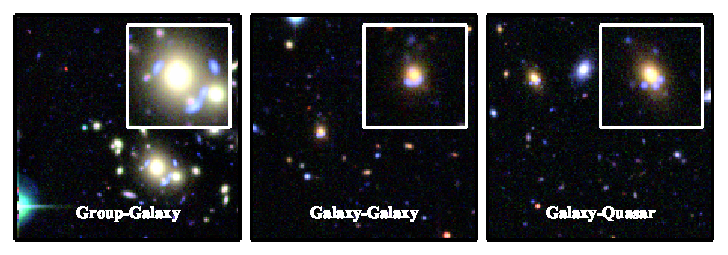
\includegraphics[scale=1.0]{sw-cfhtls-figs/sim_cgq.pdf}
\caption{ \label{fig:sim}
Examples of the three types of simulated lenses.
}
\end{center}
\end{figure*}


\subsection{Methodology}
\label{sec:simmethod}

For the purpose of generating simulated lens systems, we divide them
in to two main categories a) galaxy scale lenses b) and group or
cluster-scale lenses. We further subdivide galaxy scale lenses based on the
type of the background sources, namely galaxies and quasars. We do not simulate
group scale - quasar lenses as they are expected to be even more rare. We now
describe our procedure to generate these different types of lens systems.

\subsubsection{Galaxy-scale lenses}
\label{sect:gallens}

We begin by considering all elliptical galaxies at $z<1$ in our parent \cfhtls
catalog as potential lens candidates for the simulated sample. To avoid using a
known lens galaxy for our simulation purpose, we exclude all those galaxies
whose positions match with the lensing galaxies from the SARCS
samples within 2~arcsec (XXX check).

For each galaxy, the average number of source objects (either quasars or
galaxies) above a minimum luminosity $L_{\rm min}$ in the background that may get lensed
can be calculated as
\be
\label{eqn:nsrc}
N_{\rm src} = \int_{z_l}^\infty n_{\rm src}(>L_{\rm min},z_s)  \sigma_{\rm
lens}(\sigma_v,z_l,z_s,q) \frac{\rm d V}{{\rm d}z_s}
{\rm d}z_s
\ee
where
\be
\label{eqn:nlum}
n_{\rm src}(>L_{min},z_s)= \int_{L_{\rm min}}^\infty \Phi(L',z_s) {\rm d}L'
\ee
Here, $\Phi(L',z_s)$ denotes the source luminosity function per unit comoving
volume, $\sigma_{\rm lens}$ denotes the angular lens cross-section, which depends upon
the lens redshift ($z_l$), source redshift ($z_s$), the lens velocity
dispersion $\sigma_v$ as well as the projected axis ratio of the lens
ellipticity, $q$.

In order to calculate the lensing cross-section, we first calculate the
luminosity of each potential lensing galaxy using the photometric redshifts
($z_l$) from the LRG catalog. We use the $L-\sigma$ scaling relation from the
bright sample of \citep{Parker2005} to set the velocity dispersion of the halo
hosting the galaxy which will be later used in the model
\be
\label{magstar2}
\sigma_v=142 \left(\frac{L}{L_{*}}\right)^{1/3} \,.
\ee
We assume that the knee of the luminosity function of galaxies, $L_*$ evolves
such that there is a decline of $1.5$ magnitudes between $z=1$ to $z=0$
\citep{Faber2007}.\footnote{We anchor our $L_*$ evolution at low redshifts using the
determination of $L_*$ in the r-band by \citet{Blanton2001}. To maintain
consistency in magnitude systems, we have converted the CFHT MegaCAM magnitudes
to SDSS magnitudes and k-corrected them to $z=0.1$.}

%first calculate the
%luminosity and velocity dispersion of each potential lensing galaxy using the
%CFHT Megacam $g$ and $r$ band magnitudes along with the photometric redshift
%($z_l$) from the LRG catalog.  The Megacam magnitudes are converted to SDSS
%magnitudes\footnote{
%http://www3.cadc-ccda.hia-iha.nrc-cnrc.gc.ca/megapipe/docs/filters.html} and are
%further k-corrected to redshift $z=0.1$ \citep{Frei1994}. We assume that the
%evolution of galaxy luminosities is similar to that determined by
%\citep{Faber2007}, that is, a decline of $1.5$ in the $m_{r*}$ from redshift
%$z=1$ to $z=0$ (see Eq.~\ref{magstar}).

%\be
%\frac{L}{L_{*}}=10.0^{-0.4~(m_{r \rm SDSS}-m_{r*})}
%\ee
%
%where $m_{r*}$ is
%\be
%\label{magstar}
%m_{r*}=-20.44+ 1.5~(z_{l}-0.1) \,.
%\ee
%
%We use the $L-\sigma$ relation from
%\citep{Parker2005} to get the velocity dispersion as given in Eq.~\ref{magstar2}.

%\be
%\label{magstar2}
%\sigma=142 \left(\frac{L}{L_{*}}\right)^{1/3}
%\ee

We assume a singular isothermal ellipsoid model for each of our galaxies
\citep{Kormann1994}, such that the convergence is given by
\be
\kappa (x,y) = \frac{b \sqrt{q}}{2}\frac{1}{\left( \theta_1^2 + q^2\theta_2^2\right)^2}
\ee
Here b is called the Einstein radius, and its dependence on the velocity
dispersion of the SIE is given by
\be
b = 4\pi\,
\left(\frac{\sigma_v^2}{c^2}\right)\left(\frac{D_{ls}}{D_{s}}\right) \,.
\ee
The SIE model results in a caustic and a pseudo-caustic on the source plane:
which demarcate the regions of different image multiplicities. Parametric
solutions, $r(\theta)$ (where $\theta$ is the polar angle), for the caustics in
such a model were given by \citet{Keeton2000b}. We use these parametric
solutions to obtain the area of the lensing cross-section, $\sigma$, for every
galaxy,
\be
\sigma_{\rm lens}=\frac{b^2 q}{2} \, \int_0^{2\pi} r^2(\theta) d\theta\,.
\ee
At every polar angle we use the maximum of the radial and tangential caustic for
the purpose of calculating the cross-section.



%where
%\be
%b_I =  \sqrt{q}\, 4\pi\,
%\left(\frac{\sigma_v^2}{c^2}\right)\left(\frac{D_{ls}}{D_{s}}\right)\,.
%\ee
%Here $D_s$ and $D_{ls}$ are angular diameter distances to
%the source, and between the lens and source, respectively.

%Next, if the foreground galaxy can act as a lens and has at least one source in the
%background, then we determine a redshift ($z_s$) and $i$-band magnitude of the
%background source(s). We assume two types of background sources namely, galaxies
%and quasars. For each source, the redshift and magnitude are generated by drawing randomly from
%the following redshift and luminosity distributions. For
%galaxies, we assume the redshift distribution is

We use the results of \citet{Faure2009} to specify the source luminosity
function of galaxies. We assume that the redshift distribution of sources is
given by
\be
\label{eqn:ps}
p_s=\frac{\beta z_s^2 {\rm exp}({\frac{z_s}{z_0(m_{\rm lim})}})^\beta}{\Gamma(3/\beta)z_0^3(m_{\rm lim})}
\ee
where $\beta=3/2$ and $z_0(m_{\rm lim})=0.13m_{\rm lim} - 2.2$ and the source
counts as a function of the limiting magnitude are given by
\be
\label{eqn:ns}
n_s=\int^{m_{\rm lim}}_{-\infty} \frac{n_0 {\rm d}m}{\sqrt{10^{2a(m_1-m)}+10^{2b(m_1-m)}}}
\,,
\ee
with parameters $a=0.30$, $b=0.56$, $m_1=20$ and $n_0=3\times10^3~deg^{-2}$.

For quasars, we assume the luminosity function prescription of \citep{Oguri2010}
and adopt k-corrections by \citep{Richards2006}.
%alp=-0.5;
%kcorr=-2.5*(1 + alp)*log10(1+zz);
%Dlum=cc.Dlofz(zz)/p.hval;
%DM=5*log10(Dlum);
%Mabs=mag-kcorr-DM-25.0;
The luminosity function is expressed as
\be
\frac{{\rm d}\Phi}{{\rm d}M}=\frac{\Phi_{*}}{10^{0.4(\alpha+1)(M_{\rm abs}-M_{*})} + 10^{0.4(\beta+1)(M_{\rm abs}-M_{*})} }
\ee
where the normalization, $\phi_{*}=5.34\times10^{-6} h^3$ Mpc$^{-3}$ and break
magnitude, $M_*=-20.90 + 5 {\rm log} h - 2.5 {\rm log} f(z)$. The redshift
dependent factor in $M_*$ is given by
\be
f(z)=\frac{e^{\zeta z_s}(1+e^{\xi z_*})}{(\sqrt{e^{\xi z_s}}+\sqrt{e^{\xi z_*}})^2} \,.
\ee
We adopt the best-fit values $\zeta=2.98$, $\xi=4.05$, $z_{*}=1.60$
\citep{Oguri2010}. For the faint end slope, we use $\beta=-1.45$ whereas for
the bright end slope, we use $\alpha=-3.31$ when $z_s<3$ and $\alpha=-2.58$ at
higher redshifts, as prescribed by \citep{Oguri2010}.
respectively.


With the cross-section, and the luminosity functions specified, we calculate the
expected number of sources behind a candidate galaxy using Equation
\ref{eqn:nsrc}. We need to generate a large number of simulated lenses (larger
than the number of real galaxy lenses we expect to find in CFHTLS) in order to
use it as a training sample as well as for calibrating the performance of our
citizen scientists (see Paper I). Therefore, we artificially boost the average
number of sources by a factor (see Table~\ref{tab:thresh}, which increases the
occurrence of lensing. We draw a Poisson deviate with a mean equal to the
boosted average number of sources. If the Poisson deviate is greater than zero,
then we mark this galaxy to act as a lens galaxy. We then draw the properties of
the lensed source based on the redshift and the luminosity distribution of the
sources. The source positions with respect to the lens are drawn randomly from
an area inside the caustic.

Next, we determine properties of the background source for every lens. We follow
similar procedures for both background galaxies and quasars. We perform
ray-tracing for all of the $N_{\rm src}$ sources using the publicly available
code \gravlens \citep{Keeton2000} and choose sources that satisfy our
selection criteria. We determine fluxes of the lensed images and the total
magnification of each of the lensed source. We draw a random source for which
the flux of the second brightest lensed image and the total magnification of all
lensed images are above the thresholds given in Table~\ref{tab:thresh}.

Since we want to produce realistic looking lens systems, we simulate lenses in
each of the five \cfhtls~filters. The colors of the background source galaxies are drawn
randomly from the photometric CFHTLenS catalog
\citep{Hildebrandt2012,Erben2013}.  Similarly, we use a quasar catalog from the
SDSS Data Release 9 \citep{Paris2012} from which colors are drawn to simulate
quasar lenses. Next, we assume deVaucoleur's profile to account for the size
and shape of the galaxies. The ellipticity and the position angle (PA) are drawn
randomly between the range given in Table~\ref{tab:thresh}. The effective
radius of the galaxy is estimated from the Luminosity$-$size relation
\citep{Bernardi2003} (with a redshift scaling to account for some size
evolution) given by
\be
R_{\rm eff}= 10^{0.52} \frac{L_r^{2/3}}{{(1+z_s)}^2}
\ee
where $L_r=L_s/10^{10.2}$. On the other hand, quasars are assumed to follow a
Gaussian profile where the $\sigma$ is equated to that of the median seeing for
every filter. The median seeing values are taken from Table 4 of the official
Terapix T0007 release explanatory document \footnote{
    http://terapix.iap.fr/cplt/T0007/doc/T0007-doc.pdf}.

Once all the parameters are determined for the lens and source models, we once
again use \gravlens to generate simulated lensed images.  After accounting for the shot
noise in the lensed images and convolving them with the median seeing in each of
the filters, the simulated image is added to the real \cfhtls~image centered
on the lensing galaxy. Note that we ensure that the lensed galaxies and
lensed quasars do not have the same lensing galaxy in the foreground. Similarly,
the lensing galaxies from the galaxy-scale lenses are distinct from the central
galaxies of groups-scale lenses which are described in the following section.


\begin{figure}
\begin{center}
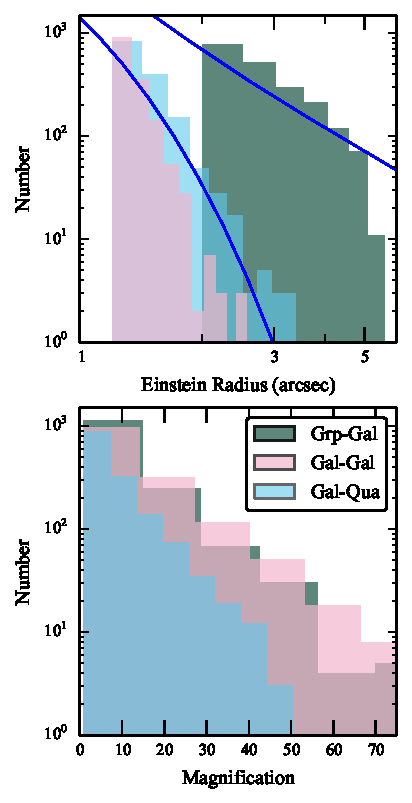
\includegraphics[scale=1.2]{sw-cfhtls-figs/distrib_remu.pdf}
\caption{ \label{fig:remudist}
Einstein radius distribution for all types of lenses. The dashed-dotted (blue)
curves show the theoretical prediction assuming an SIS model at galaxy-scales
and a total (NFW+Hernquist) model at groups-scales taken from \citep{More2012}.
%{\bf fix the normalization}
}
\end{center}
\end{figure}


\begin{table}
\begin{center}
\caption{ \label{tab:thresh}
Thresholds used in the selection of the simulated lenses. }
\begin{tabular}{l l l l l}
\hline
Name  &  \multicolumn{2}{c} {Gal-Gal (Grp-Gal)}  & \multicolumn{2}{c}{Gal-Qua} \\
      & min  &  max  & min & max \\
\hline
\hline
Source Redshift  & 1.0 & 4.0  & 1.0  & 5.9 \\
Source Flux      & 21.0 & 25.5 & 21.0 & 25.5 \\
Source ellipticity & 0.1 & 0.6 & - & - \\
Source PA & 0 & 180 & - & - \\
Lens Redshift  & - & 0.9  & -  & 0.9 \\
Lens shear strength &  0.001 (-) & 0.02 (-) &  0.001 & 0.02 \\
Lens shear PA &  0 (-) & 180 (-) & 0 & 180  \\
Einstein radius (arcsec) & 1.2 (2) & 5 (-) & 1.2 & 5 \\
\hline
boost factor     & $=$100 (40)  &  & $=$1200 & \\
Image Flux$_{\rm 2B}$ & $>$23  & & $>$23 & \\
Image Flux$_{\rm tot}$ & $<$19 & & $<$20 & \\
\hline
\end{tabular}
\end{center}
a) () -- corresponds to quantities used for Grp-Gal scale lenses, if they
are different from Gal-Gal.
b) $_{\rm 2B}$ --  the second brightest lensed image.
c) $_{\rm tot}$ -- total flux integrated over all of the lensed images.
d) All fluxes are in AB mag. PA is in degrees measured East of North.
\end{table}

\subsubsection{Groups-scale lenses}

At group or cluster-scales, the mass distribution is more complex. The
convergence in the inner regions, which are typically responsible for the
multiple lensed images, arises from not only the brightest group galaxy (BGG) at
the center, but also has contribution from the dark matter component as well as
the satellite galaxies \citep{Oguri2005,Oguri2006}. We generate a basic group
catalog based on the magnitudes and photometric redshifts available for the
\cfhtls. We select all galaxies with 10$^{10.8} M_\odot$ as plausible BGGs. We
select the member galaxies such that their photometric redshifts are within
$\delta z = 0.01$ of the BGG and within an aperture of $250$~Kpc. If another BGG
is found with the aperture, then the fainter BGG is removed from our list of
BGGs.

\begin{figure*}
\begin{center}
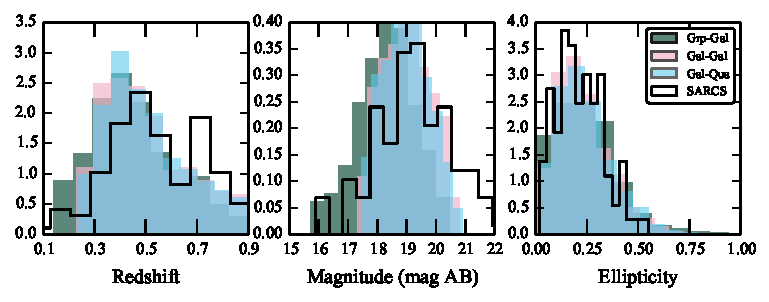
\includegraphics[scale=1.3]{sw-cfhtls-figs/lensprop.pdf}
\caption{ \label{fig:lensprop}
Distributions of properties of the lensing galaxies of the simulated
sample compared to the known lens sample SARCS. %(XXXX confirm what's being plotted? which band - i?)
}
\end{center}
\end{figure*}

We assume a constant mass-to-light ratio of $3 \times 0.7$~h~$M_{*}/L_{*}$, to
convert the BGG luminosity to a stellar mass estimate. The stellar mass$-$halo
mass relation \citep{Behroozi2013}, including random scatter, is then used to
calculate the halo mass for the lens. We adopt an NFW density profile for the
underlying dark matter halo. Given the halo mass, other key parameters such as
the scale radius ($r_s$) and the density at the scale radius ($\rho_s$) can be
determined for an NFW profile. In addition, we adopt an isothermal ellipsoid
model for the BGG and members whenever the ellipticities are available from the
galaxy catalog (else we use an isothermal sphere).

We calculate the luminosity and velocity dispersion for the BGG and each of the
member galaxies following the same prescription as in
Section~\ref{sect:gallens}. To calculate the average number of sources that get
lensed by such a system, we need to calculate the lensing cross-section for each
of these potential lensing groups. The complexity in the lens models makes it
analytically intractable to calculate the size of the caustics\footnote{The lens
mass distribution determines size and shape of the caustics. Any source
located within the caustics will form multiple lensed images which is the
criteria for strong lensing. To further understand caustics, see XXX.}.
Therefore, we generate the caustics numerically using \gravlens and then
determine the area covered by the caustics. We consider only galaxies as our
background source population since group or cluster-scale quasar lenses are not
expected to be extremely rare in the \cfhtls (check XXX).  Following the same procedure
as described in Section~\ref{sect:gallens}, we calculate the number of galaxies
expected to lie behind every potential lensing group (see Eq.~\ref{eqn:nsrc}).
As before, for each background galaxy within the lens cross-section, a redshift
and an $i$-band magnitude is determined by drawing galaxies randomly from the
respective distributions (see Eqs.~\ref{eqn:ps}-\ref{eqn:ns}).

All those groups that are found to have no background galaxies within the
cross-sectional area are rejected and the rest are included as potential lenses.
As mentioned earlier, we artificially boost the total number of sources behind
every lens but ensure that (check XXX) the statistical properties such as the profile of the
image separation distribution are not affected (see \Fref{fig:remudist}). We
follow the same procedure and apply the same thresholds to determine properties
of the lensed galaxies for every lens as are described for galaxy-galaxy lenses
in the previous section. The simulated lensed images are then added on top of
the real \cfhtls~images with the BGGs as the center.

% % % % % % % % % % % % % % % % % % % % % % % % % % % % % % % % % % % % % % %

\subsection{Simulated Lens Sample and Catalog Description}

In this section, we describe some of the properties of our simulated sample for
each of the three types of lens samples.

\Fref{fig:remudist} shows the Einstein radius distribution for the
galaxy-scale (dashed for background quasars and dotted for background galaxies)
and groups-scale simulated lenses. For comparison, we show the expected
distributions (blue dashed-dotted curves) for an SIS-like density profile at
galaxy-scales and an NFW+Hernquist profile at groups-scales. The
theoretical curves are taken from \citep{More2012} wherein the models are
explained in detail. We note that the model we adopt at groups-scale also
includes SIS or SIE components for the group members unlike the theoretical
prediction. The theoretical curves have arbitrary normalizations.

We show the redshift, magnitude and ellipticity distributions of the lensing
galaxies in the three panels of \Fref{fig:lensprop}, respectively. We also show
the distributions of respective properties of the SARCS lenses from
\citep{More2012} for comparison with arbitrary normalizations. We note the
qualitative similarities between the simulated and the real lens samples.

%Similarly, we show the ellipticity and the position angle of the simulated lens
%galaxy population extracted from the T0007 release of the \cfhtls~catalogs in the
%left and right panels of \Fref{fig:lensprop}, respectively. As before, the
%dashed-dotted (blue) curves show the same distribution for the SARCS lens
%population with arbitrary normalization \citep{More2012}.

%We show the source redshift and magnitude distributions for each of the three
%lens samples in the left and right panels of \Fref{fig:szmdist},
%respectively. The peak of the source redshift distribution both for the galaxies
%and quasars is known to be between $2<z<3$ from various lens samples (add
%references XXX). This consistent with our simulated sample as expected. The
%magnitude distribution of the simulated sample, on the other hand, is
%specifically tailored to the requirements of \sw.  The goal was to generate a
%lens sample that has a fair balance of both bright and faint lensed images since
%the training sample should neither be too easy nor too difficult for the citizen
%scientists.

We produce catalogs with lens and source properties for each of the three types
of lenses. These catalogs are available from
https://github.com/anupreeta27/SIMCT. The catalogs typically have lens
position, redshift, magnitudes, Einstein radius, ellipticity (whenever
available) and shear (for galaxy-scale lenses only). For the background
sources, we provide the offset from the lens center, redshift, magnitudes,
total magnification, number of lensed images. Additionally, when possible,
ellipticity and effective radius of the background galaxies have also been
provided.

% % % % % % % % % % % % % % % % % % % % % % % % % % % % % % % % % % % % % % %

\subsection{Limitations of the simulated sample}
The simulated lens sample, although realistic, is not perfect, due to the
simplicity of the lensing models and our limited understanding of the
uncertainties in the parameters for the models. Comments from citizen
scientists were very helpful in order to sort some of these failures. Here, we
describe some of the cases or aspects in which the simulations were known to
have failed (or appeared unrealistic). This typically happens for a small
fraction of the simulated images (roughly 5 percent of
the cases)\footnote{Based on the hashtag simfail in the discussion forum
TALK.}.

The parameters required by various scaling relations and the models primarily
depend on the photometry of the galaxies, groups and quasars detected in the
survey. For galaxy-scale lenses, the lensing galaxies at higher redshifts or
which are fainter have poor photometric redshift measurements. Consequently
these galaxies are assigned a wrong luminosity and velocity dispersion
estimates, which sometimes result in simulated lenses which look implausible.
For example, the lensed images for some of the failed simulations have larger
image separation than expected given the visual priors from the galaxy.

At group-scales, the photometric and redshift estimates are used when define
the group membership. Therefore, errors in redshift estimates generate galaxy
groups with BGG or member galaxies with dissimilar properties. In some cases,
low redshift spiral galaxies have been incorrectly assigned high redshift.
Spiral galaxies are typically less massive and low redshift spiral galaxies are
unlikely to act as gravitational lenses. Hence, some of the simulated lenses
were not as convincing.

We also use a single Sersic component to describe the light profiles of
background galaxies. This is clearly not the most accurate description for
galaxies, especially, star-forming galaxies which form a significant fraction
of the lensed galaxy population. Star-forming galaxies have complex structures
such as star forming knots, spiral arms, bars and disks. The simulated lensed
images do not display these features.

%magdiff=5*0.1;
%zdiffq=0.1;

%
%\begin{figure}
%\begin{center}
%\includegraphics[scale=0.95]{sw-cfhtls-figs/distrib_reff.eps}
%\caption{ \label{fig:reffdist}
%Distributions of magnification (left) and source effective radius in units of
%pixel (right).
%}
%\end{center}
%\end{figure}

% % % % % % % % % % % % % % % % % % % % % % % % % % % % % % % % % % % % % % %

\section{Training sample: Duds and False positives}
\label{sec:dfp}

Citizen scientists not only need training to identify gravitational lenses, but
also to reject images which either contain impostors or have no lenses. Hence,
in addition to the simulated lenses, we added a sample of duds and false
positives to the training sample. Duds are images which have been visually
inspected by experts and confirmed to contain no lenses.  False positives (FPs)
are systems which look like lenses but are not, for example, spiral galaxies,
starforming galaxies, chance alignments of features arranged in a lensing
configuration and stars.

We selected a sample of 450 duds for the \StageOne classification in \sw
and a sample of 500 false positives for the \StageTwo inspection. The
sample of false positives was selected from the candidates which passed
the \StageOne of \sw. We note that this is the first time, we have a
systematically compiled sample of visually inspected false positives by
the \sw volunteers and categorized by the science team. The data products are
available at http://spacewarps.org/\#/projects/CFHTLS/. Such a sample is
tremendously helpful for training and understanding performances of
various lens finding algorithms \citep{Chan2014}.

\begin{figure}
\begin{center}
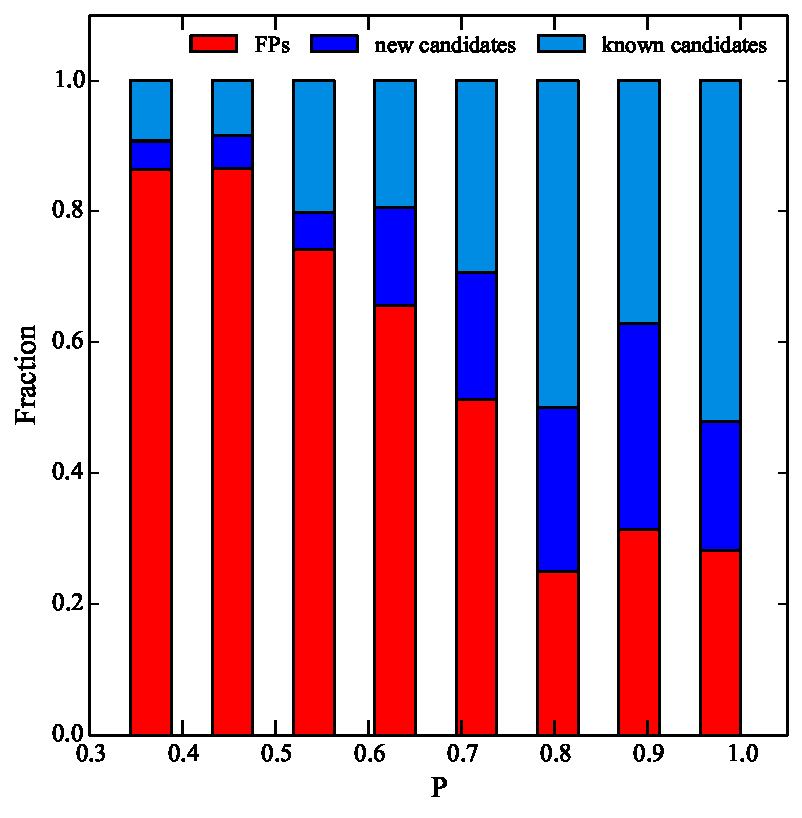
\includegraphics[scale=0.6]{sw-cfhtls-figs/cand_fp_P_frac.pdf}
\caption{ \label{fig:stackP}
Distribution of different types of candidates as a function of the posterior
probability P. The types of the candidates are the FPs, the new candidates and
the known candidates. The new and known candidates have higher detection rate
for higher values of P, as expected.}
\end{center}
\end{figure}

%%%%%%%%%%%%%%%%%%%%%%%%%%%%%%%%%%%%%%%%%%%%%%%%%%%%%%%%%%%%%%%%%%%%%%%%%%%%%%

\section{Methodology to produce the \sw-\cfhtls Lens Sample}
\label{sec:swap}
The \sw works as a single unified neural network which uses the method of visual
inspection to find gravitational lenses. The volunteers are shown images at two
stages. At \StageOne, volunteers are requested to undertake a rapid inspection to
select lens candiates ranging from possible lenses to almost certain lenses. At
\StageTwo, volunteers carefully inspect the candidates from \StageOne and select only
promising lens candidates. A daily snapshot of classifications performed by
volunteers are provided to the science team every night. This daily batch is
analyzed by the Space Warps Analysis Pipeline (SWAP). The philosophy and the
details of SWAP are described in detail in Paper I, here we briefly summarize
how it works.

Each subject (or image cutout) is assigned a prior probability of
$2\times10^{-4}$ to contain a lens system. Every volunteer or classifier
is assigned an agent characterised by a $2\times2$ confusion matrix,
which quantifies the volunteer's ability to correctly classify an image
to contain ($P_L$) or not contain a lens system ($P_D$). The values of
the confusion matrix are determined based on the performance of the
volunteer on the training sample, specifically, $P_L$ (and $P_D$) is
determined based on the fraction of simulated lenses (and duds)
correctly classified. After every classification, the agent updates the
prior probability of the classified subject based on the classification
and the volunteer's confusion matrix, according to the Bayes theorem.
Note that the volunteer's confusion matrix is updated after the
classification of every training image. Threshold values for the
probabilities to accept (or reject) a subject  if it contains (or doesn
not contain) a lens can be chosen in SWAP. Those images which cross
these threshold values are retired and are not subsequently shown to the
volunteers, so that volunteers can use their time efficiently to
classify previously unclassified subjects.

SWAP was run nightly during \StageOne in order to retire subjects and inject new
ones in to the classification stream. The subjects that passed the acceptance
threshold at the end of \StageOne are served again at \StageTwo for careful
reinspection. Each subject, after \StageTwo, has an associated posterior
probability P. In the ideal case, all images containing lenses will have high P
values and those without lenses will have low P values. In practice, we expect a
small fraction of the real lenses (or non-lenses) to be assigned low (or high) P
values and thus, decreasing the completeness (or purity) of the final lens
sample.  As this is the first candidate search with \sw, we want to find a
threshold P value which will result in acceptable levels of completeness and
purity of the final sample of lens candidates.

We decided to inspect the top few hundreds of images from a catalog of
descending P values as a reasonable sample size for visual inspection.
We find a total of 665 subjects with P$>0.3$ in the catalog. These
images were then visually inspected by three lens experts (AM, AV, PJM).
The images are assigned grades on a scale of 0 to 3, thus dividing the
subjects into candidates that almost certainly do not contain a lens,
possibly a lens, probably a lens and almost certainly a lens,
respectively. The final sample of \sw-\cfhtls lens candidates (see
\Sref{sec:swlens}) is produced by selecting candidates above some
threshold on the averaged grades.


%%%%%%%%%%%%%%%%%%%%%%%%%%%%%%%%%%%%%%%%%%%%%%%%%%%%%%%%%%%%%%%%%%%%%%%%%%%%%%
\section{Results}
\label{sec:results}

\subsection{\sw-\cfhtls Lens Sample}
\label{sec:swlens}

In this section, we describe the \sw-\cfhtls lens sample (henceforth,
called the \sw lens sample). We find a total of XXX (and XXX new)
candidates with averaged grade $0<$G$<1.3$ (low probability sample)
which means at least one of the inspector gave a grade of 1 and the
maximum grade given by all three inspectors was 1\footnote{If grades
from the inspectors were found to be discrepant by 2 or more, these were
discussed and re-graded to resolve the discrepancy}. Further information
on the low probability sample such as their positions and images are
available at http://spacewarps.org/\#/projects/CFHTLS/. 

There are a total of XXX candidates with $1.3\le$G$<2$ (medium
probability sample) out of which 30 are new. These grades suggest that,
most of the times, at least one of the inspectors gave a grade of 2 and
the maximum grade by all of the inspectors was below 2. Among our high
probability sample (G$\ge$2), there are a total of XXX candidates out of
which 28 are new which means at least two of the inspectors gave a grade
of 2 or higher. To avoid duplication, further information on \sw
candidates that were previously identified in the literature is
available at http://spacewarps.org/\#/projects/CFHTLS/ whereas the new
lens candidate sample of medium-high probability is presented in this
paper (see \Sref{sec:results:newcand}).

In Table~\ref{tab:stats}, we give overall statistics of the systems detected at
\StageOne and \StageTwo. We give the total number of detections of the known lens
candidates, known lenses and the new lens candidates at each stage.  We also
show their fractions with respect to the total number of lens candidates found
at these stages. We note that most (XXX check) of the confirmed lenses found at
\StageOne are also recovered at \StageTwo whereas a small fraction of the known
lens candidates are rejected at \StageTwo. Also, the sample of new lens
candidates increases the sample of \cfhtls lens candidates by over 50\%.

In \Fref{fig:stackP}, we plot the distribution of false positives and the high
probability lens candidates, categorized by the lens experts, as a function of
the P value assigned by SWAP at the end of \StageTwo. On average, the fraction of
lens candidates is indeed an increasing function of P. This shows that the \sw
generated P values for the subject are roughly correlated with the expert grades
albeit with quite some scatter.  We note that from P$\sim$0.75 onwards to lower
P values, the fraction of false positives starts to exceed the fraction of real
lens candidates. This could be a good threshold to choose to maximize the purity
of the final sample. However, the choice of P$=$0.3 as the threshold gives a
more acceptable completeness of XXX for our sample which combined with expert
grading allows us to achieve further purity of our sample.
%{\bf AM: give some numbers for the completeness/purity ? I will check what grades we gave to the stage 2 detected KLs and comment on it.}


\begin{table}
\begin{center}
\caption{ \label{tab:stats}
Statistics of detections in \sw }
\begin{tabular}{l l l l l}
\hline
   &  \multicolumn{2}{c} {\StageOne}  & \multicolumn{2}{c}{\StageTwo} \\
      & KC  &  KL  & KC & KL \\
\hline
\hline
Number  & 128 & 34 & 107  & 34  \\
Percentage  & & & & \\
of recovery & 29 & 58 & 25 & 58  \\
P$_{\rm thresh}$ & 0.95 & 0.95 & 0.3 & 0.3 \\
\hline
   &  \multicolumn{2}{c} {\StageTwo}  &   & \\
      & NC  &  AC  &  & \\
\hline
\hline
Number  & 58 & 168 &  & \\
Percentage & & & & \\
of detection & 12 & 34 &  & \\
P$_{\rm thresh}$ & 0.3 & 0.3 &  & \\

%% ####stage1
%% cand 128/436
%% conf  34/59

%% ####stage 2
%% sarcs conf 18/26
%% sarcs cand  55/106
%% RF conf 16/33
%% RF cand  52/330

\hline
\end{tabular}
\end{center}
{KC}-- Known lens candidates \\
{KL}-- Known lenses \\
{NC}-- New lens candidates  \\
{AC}-- All (known and new) lens candidates  \\
P$_{\rm thresh}$ -- systems with P above this threshold are selected \\
Note: For KC and KL, Percentages are with respect to the known
population whereas for NC and AC, percentages are with respect to the
total population of lens candidates. \\
\end{table}

% % % % % % % % % % % % % % % % % % % % % % % % % % % % % % % % % % % % % % %

\subsection{New lens candidates from \sw}
\label{sec:results:newcand}

We give basic information about the final sample of 58 new lens
candidates (medium-high probability) found by \sw in
Table~\ref{tab:swcands}. We report the candidates with a \sw ID and Name of the
lens system. We give their positions (Ra, Dec), photometric redshift
($z_{phot}$), $i$ band magnitude of the lensing galaxy, averaged grade G from
the lens experts, zoo ID (identifier used in TALK), P
value at \StageTwo and a visual categorization of type of lensed images and the
lensing galaxy in the Comments column in Table~\ref{tab:swcands}. Whenever
available the lens properties are taken from the \cfhtls photometric catalog
\citep{Coupon2009} otherwise the reported lens galaxy positions are measured
manually. The visual categorization of the lens type is only suggestive and the
explanation of the notations in the Comments column is given at the bottom of
the table.

We show images of our new sample in \Fref{fig:lc} which is arranged
first in the decreasing order of their grades and then increasing order
of their positions. As the first lens search was a blind search with no
preselection of candidates from any algorithm, we find various types of
lenses, as expected from such a search. The final sample consists of
both galaxy and groups-scale lens candidates. There are detections of
elongated arcs and some interesting point-like quasar lensed images.
Most of them are brighter in bluer $g$ band but some candidates brighter
in the redder $i$ band are also found. Since robotic lens searches often
look for blue colored lensed features, they are very much likely to miss
such interesting lens candidates.  We did not find any examples of
exotic lens candidates from the visually inspected P$>0.3$ sample. There
may be some interesting candidates lurking in TALK but these will have
to be sifted through ({\bf is there someone actively looking into this
whose work should be referred here ?}). 

The new \sw lens sample presented here shows the advantages of having
citizen scientists find lenses through visual inspection. An algorithm,
by definition will find objects that adhere to a selection criteria that
uses either geometry or flux information from an image. On the other
hand, citizen scientists can do amazing amount of interpolation or
extrapolation over the basic selection criteria provided to them. 
For example,  the lower blue arc in SW7 is split by a small red galaxy.
An algorithm typically fails to detect such arcs because the arc is
broken into smaller arclets which then falls below the minimum length or
area allowed for an arc to be detected typically. Human brains have no
problem in interpolating over the broken blue arc over the red galaxy
and understand that it is a single long arc. The system SW19 has
point-like lensed images which cannot be detected by arc finding
algorithm whereas the ring finding algorithm may miss this because of
atypical color and structure of the galaxy. 

The power of citizen scientists lies in the high dynamic range that
allows us to detect systems with very from small-to-large arcs, from
highly compact-to-low surface brightness images, from round and
point-like to elongated and curved images, from blue-to-red, from
regular-to-exotic kinds of lenses while keeping the false positive rate
comparatively low. Further detailed qualitative and quantitative
analysis of the properties of the entire \sw sample (new and previously
identified candidates) and the mass modelling analyses for the new
candidates will be presented in a subsequent \sw paper, Paper III.


%{\bf CHECK FOR STAGE 1 -- COMPLETENESS OF KNOWN LENSES and P value comparison, 

% what about the duplicate lenses near the borders -- stats on those?  

% check the detection plot of arc mag / Reinst and find out why some of
%the bins have unexpected results. 

%check if some candidates were detected because they were hidden
%underneath the sims ie. from the D11;
%}


\begin{figure*}
\begin{center}
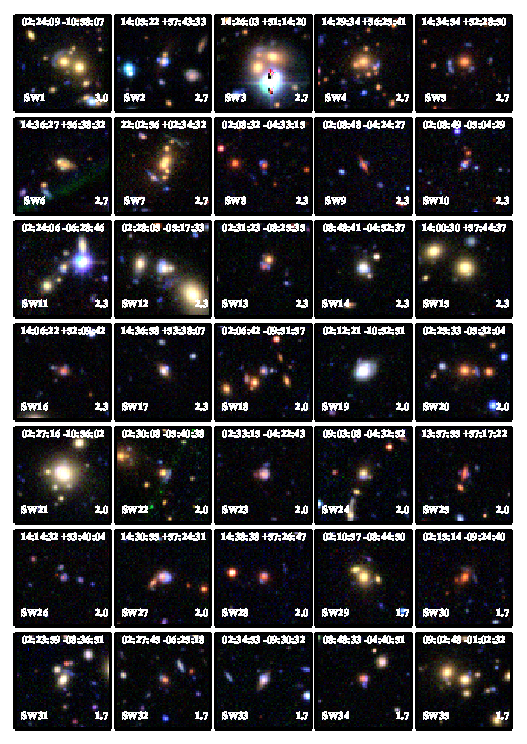
\includegraphics[scale=1.9]{sw-cfhtls-figs/lenscandfin.pdf}
\end{center}
\end{figure*}

\begin{figure*}
\begin{center}
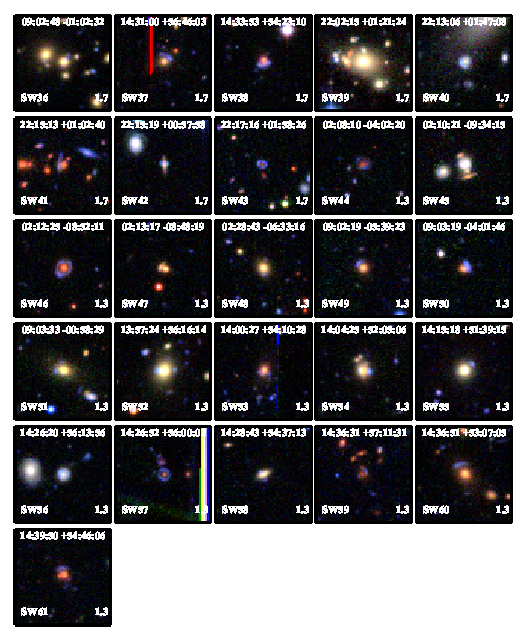
\includegraphics[scale=1.9]{sw-cfhtls-figs/lenscandfin_1.pdf}
\caption{ \label{fig:lc}
The new \sw lens candidates with expert grade G$>=$1.3. The images are
30\arcsec on the side.
}
\end{center}
\end{figure*}
% % % % % % % % % % % % % % % % % % % % % % % % % % % % % % % % % % % % % % %

\subsection{Measurements of properties of the lens and the lensed images}
\label{sec:results:meas}

In the subsequent sections, we make comparison of various properties of the lens
candidates. In this section, we describe how we extract these properties, namely,
the lens redshift, the Einstein radii and the total flux of the lensed images or
arcs.

We use the publicly available redshifts for the lens galaxy from the
\cfhtls photometric catalogs \citep{Coupon2009}. The total flux of the
lensed image or arc is measured in the $g$ band but the adopted method
is different for different samples. For the simulated sample, we
multiply the magnification of the second brightest image with the source
magnitude. For the \rf sample, the arcs are detected in the scaled
difference image between $g$ and $i$ bands where the lensing galaxy is
subtracted \citep[for details, see]{Gavazzi2014}. Here, we use the flux
of the lensed images measured by {\sc sextractor} from the scaled
difference image, that is, $g-\alpha i$ and convert it to the $g$ band
flux using mean colors of the foreground and background population. For
the \af and the \sw sample, we integrate the flux in the image pixels
identified by \af or {\sc sextractor}.


The Einstein radius ($R_{\rm E}$) is also measured differently for
different samples. For the galaxy-scale lenses in the simulated sample,
we use the value of the input lens model parameter for the $R_{\rm E}$.
For groups-scale lenses, since the lens model is multi-component, we
need to determine the $R_{\rm E}$ from the image positions. We use those
pairs of lensed images that have the smallest and the largest angular
separations. The $R_{\rm E}$ here is then half of the averaged values of
these angular image separations.  For the \rf sample, we use the peak
position of the lensed images measured by running {\sc sextractor} on
the scaled difference image. We calculate the image separation from the
lens center as an estimate of the $R_{\rm E}$. For the \af (SARCS)
sample, we use the same definition as above except that the peak
position is identified either by the \af or manually. For the \sw lens
sample, the same definition is used where the peak positions are
identified either with \af or {\sc sextractor}.


% % % % % % % % % % % % % % % % % % % % % % % % % % % % % % % % % % % % % % %

\subsection{Recovery of known lens samples from the \cfhtls by \sw}
\label{sec:results:known}

We determine what fraction of the known sample of lenses are recovered
by \sw. Note that this sample corresponds to the \rf and \af samples
combined, as mentioned in \Sref{sec:data:kls}. In Table~\ref{tab:stats},
we show that $\sim$~25\%-30\% of the known lens candidates and
$\sim$~60\% of the known lenses are found at \StageOne and \StageTwo in
\sw. The left and the middle panels of \Fref{fig:compre} show the
fraction of detections as a function of arc magnitude and the Einstein
radius of the lens systems for the known confirmed lenses and lens
candidates. As expected, we find that systems with brighter images
and/or with larger Einstein radii are detected more often in \sw.

We find that most of the confirmed lenses and candidates that are missed
by \sw are systems with fainter arcs and smaller Einstein radii and they
come from the \rf sample. The main reason why \rf found such candidates
is because their team used lensing galaxy-subtracted images to detect
the presence of the lensed images both during the automated
object-finding phase and during the visual inspection and classification
of their candidates. This approach naturally improves the detection
efficiency at smaller Einstein radii and for fainter systems. The \sw
volunteers were not shown any galaxy-subtracted images. However, showing
galaxy subtracted images might be a better strategy to adopt for future
lens searches at galaxy-scales with \sw. In the Discussion
\Sref{sec:fn}, we further explore and discuss why some of the confirmed
lenses are missed by \sw.

\begin{figure*}
\begin{center}
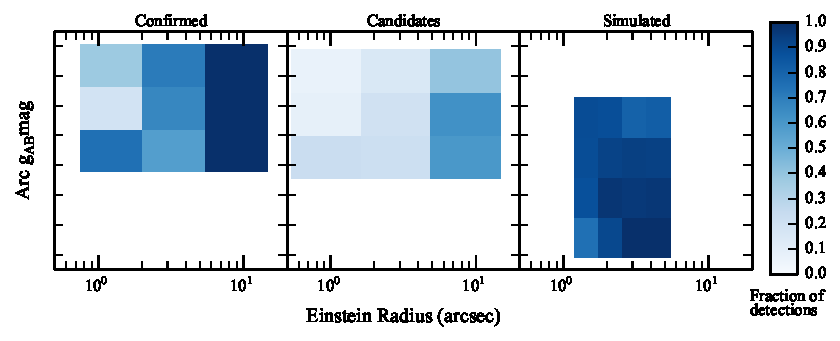
\includegraphics[scale=1.0]{sw-cfhtls-figs/comp_reinst_mag.pdf}
\caption{ \label{fig:compre} Fraction of lens candidates recovered by \sw as a
function of the arc magnitude ($g$ band) and the Einstein radius for three lens
samples, namely, the known lenses, the known lens candidates and the simulated
sample. }
\end{center}
\end{figure*}


% % % % % % % % % % % % % % % % % % % % % % % % % % % % % % % % % % % % % % %
\subsection{Image separation distribution}
\label{sec:results:isd}

The distribution of image separations (i.e. twice the Einstein radius)
can be used to probe the average density profile of the lens population
\citep{Oguri2006,More2012}.  However, the lens sample found by the \af
may have incompleteness as a function of the image separation. Thus, the
lack of understanding of the selection function of the lens sample may
affect the constraints on the density profile. A blind lens search done
by visual inspection alone, for example, through \sw citizen scientists may find
lenses missed by the \af search and thereby, improve completeness.

Indeed, we have find several new lens candidates that were not known
before. In \Fref{fig:isd}, we show the image separation distribution for
the known sample (green), for the \sw identified (known and new) lens
sample (blue) only and combined known with the new \sw lens sample
(magenta). It is interesting to note that both these samples have very
similar profiles and thus, the profile of the combined sample has not
changed much. This implies that previous constraints on the image
separation distribution are robust and the \af selected sample does not
suffer from significant incompleteness for medium to large Einstein
radii. This is the regime that probes density profiles of galaxy groups
to clusters.
%%{\bf AM: understand what Phil wanted to say about AF's (in)completeness}

In the figure, we also show for comparison the theoretical predictions
corresponding to three density profiles, namely, isothermal sphere (IS),
NFW \citep{Navarro1997} and Total profile which has NFW and Hernquist
profiles combined with an adiabatically contracting model for dark
matter component \citep{Gnedin2004}. These curves are taken from
\citet{More2012} which gives details of the calculation of these
predictions.  With the updated sample of lens candidates, we confirm our
previous prediction that the mass density profiles of galaxy groups is
indeed similar to the Total profile.

%%%%%%%%%%%%%%%%%%%%%%%%%%%%%%%%%%%%%%%%%%%%%%%%%%%%%%%%%%%%%%%%%%%%%%%%%%%%%%

\begin{figure}
\begin{center}
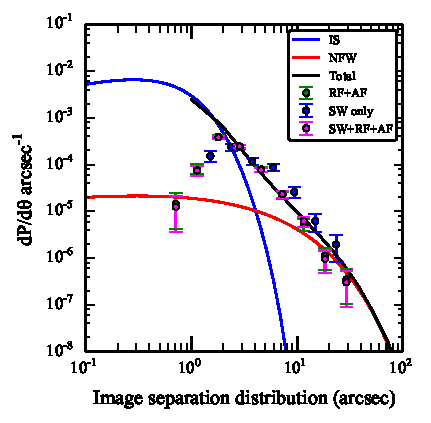
\includegraphics[scale=1.2]{sw-cfhtls-figs/isd_cfhtls_sw.pdf}
\caption{ \label{fig:isd} Image separation distribution. Comparing theoretical
predictions (solid curves) with the \cfhtls known lens samples (green)
and the combined sample of known and \sw lens candidates (magenta). The
sample of new and the known lens candidates discovered from \sw alone is
shown in blue. The new updated profile of the isd (magenta) is
consistent with our previous measurements and strengthens our conclusion
that the average density profiles of the lenses are similar to the Total
profile.}
\end{center}
\end{figure}

\section{Discussion}
\label{sec:discuss}

Finding gravitational lenses is a difficult and complex task. No one
method is perfect. Each method has some advantages over the other. It
may be the case that a single method may never be the best method for
optimising completeness and purity. Visual inspection will likely be
required for pruning candidates at some stage of lens candidate
selection even in the future. Therefore, we would like to understand how
best we should combine the strengths of robots and humans to optimize
the lens finding method.

In this section, we first compare the lens candidates found by
\sw and the lens finding robots and then attemp to understand why each
method failed to detect lenses from the other sample.

\subsection{Comparison of the \rf, \sw and \af samples}
Here, we compare the properties of the lens candidates from each sample
to understand if there are any clear differences between them. We
consider the lens redshift, the total flux of the lensed images and the
Einstein radii of the systems for this purpose.

In \Fref{fig:zlmgre}, we show the lens redshift and the arc flux
measured in $g$ AB mag as a function of the Einstein radius for the \rf
(green), the \af (red) and the \sw sample (new candidates only in blue
and known candidates as black circles). We note that the errors on the
redshift measurement should not be too different across the samples
since they are measured by a single method. However, the error on the
total flux of the lensed images are likely to be different across the
samples and the types of systematics are also different.  We have not
attempted to quantify these errors in this work. With that caveat, we
find that the \sw candidates sample is broadly similar to the
robotically found lens candidates in terms of the flux of the lensed
images or the redshift of the lensing galaxies.

Since \sw is visual based search, it is difficult to detect many lens
candidates with small $R_{\rm E}$ in the presence of a bright lensing
galaxy. While this is true for algorithms too, the \rf team adopted a
different method to circumvent this problem whose goal was to find
galaxy-scale lenses which have small $R_{\rm E}$. The \rf sample is
generated by working with lensing galaxy $-$subtracted images and this
led to increased detections of small image separation candidates. The
\sw lens search did not show any galaxy subtracted images and hence,
this results in a quantitative difference between the \sw and the \rf
sample as a function of $R_{\rm E}$.

The \af, on the other hand, is capable of finding smaller image
separation lenses but a lower limit on $R_{\rm E}$ was imposed by the
\af team to simplify the selection function of their sample. Thus, we
can compare the \sw and \af samples at about $R_{\rm E}>2\arcsec$. There
is a good overlap between the two samples given that most of these are
candidates and could turn out be not lenses. We again caution the
readers that the uncertainties on the measurements are not quantified
and may change the results to some extent.

The properties considered here do not show any clear differences between
the types of lenses being found by each method. Other properties such as
the flux of the lensing galaxies and the surface brightness of the
lensed images may be useful in showing some qualitative differences but
this is beyond the scope of our current analysis. A more detailed and
accurate analysis is deferred to the future.
%{\bf check out of the 55 promising \af how many are missed by \sw ?}

Lastly, in \Fref{fig:stackremg}, we show the relative distribution of
number of candidates from each sample as a function of the Einstein
radius and arc magnitude. The light blue color shows the overlap between
the \sw and the \rf samples and the purple color shows the overlap
between the \sw candidates and the \af samples. As noted earlier, the
\rf dominates the small $R_{\rm E} (<2\arcsec)$ range although \sw does
find modest number of candidates in this range. At larger $R_{\rm E}$,
\sw sample begins to dominate and is comparable to the \af sample.  As a
function of the arc magnitudes, all three samples have detections at all
magnitudes and median magnitudes for all samples is around 24.5.
Relatively, the \rf sample spans a narrower range compared to the \sw
and \af sample. However, this can be verified only after understanding
and accounting for the systematic uncertainties in our measurements.

\begin{figure}
\begin{center}
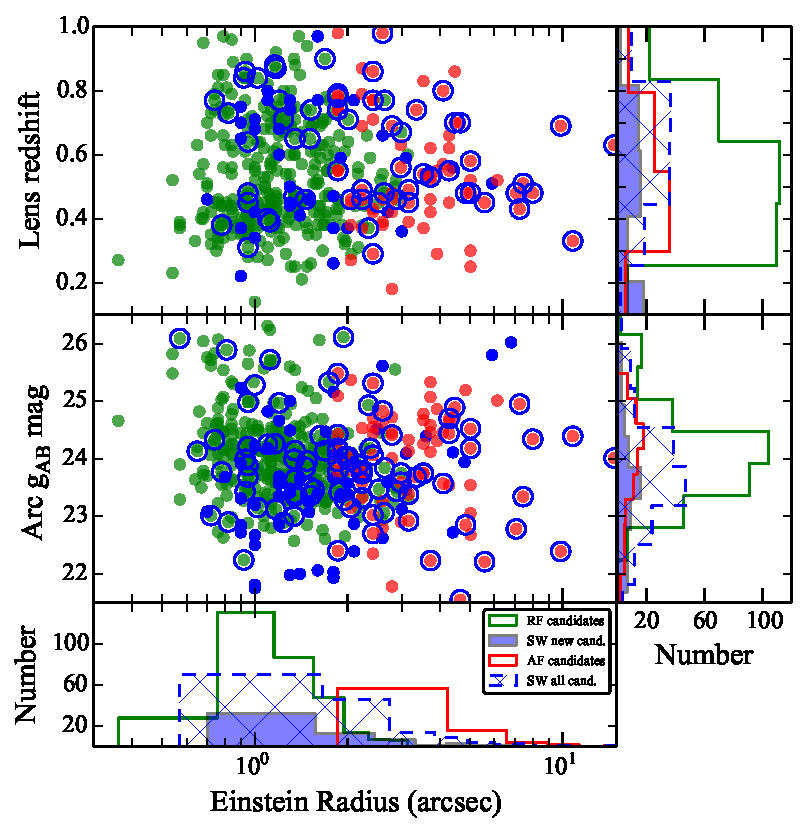
\includegraphics[scale=0.65]{sw-cfhtls-figs/zl_mg_re.pdf}
\caption{ \label{fig:zlmgre}
Comparison of the lens redshift and the arc magnitude with the
Einstein radius for all of the three lens samples, namely, the \rf (green dots),
\sw (known candidates$-$black circles and new candidates only$-$blue dots)
and \af (red dots). Alls samples have broadly similar properties.}
\end{center}
\end{figure}

\subsection{Why \sw candidates were missed by lens finding robots?}
We rerun the \rf and \af on images centered on the new \sw candidates to
trace and understand at what stage the algorithm failed to detect them.

First, we rerun \rf on the new \sw sample. At the beginning, a galaxy
catalog is generated based on magnitude, redshift and SED type
\citep[see]{Gavazzi2014} to select galaxies which are most likely to act
as lenses. We find that about 40\% of the new \sw candidates fail to
meet this initial selection criteria, for example, SW1, SW13, SW19, SW22, SW26
and SW29.  All of the lensing galaxies are bright enough to satisfy the
$i<22$ criterion. However, some of them have a bright companion galaxy,
some of them do not look like E/S0 type galaxies and some are edge on
galaxies.

%{\bf can we say something qualitatively for why these were missed? there are a few which look regular galaxies so which criteria are they failing??}
%% 13 are under mask so no photoz, 10 have photoz (z>0.2 except for 1).

\begin{figure*}
\begin{center}
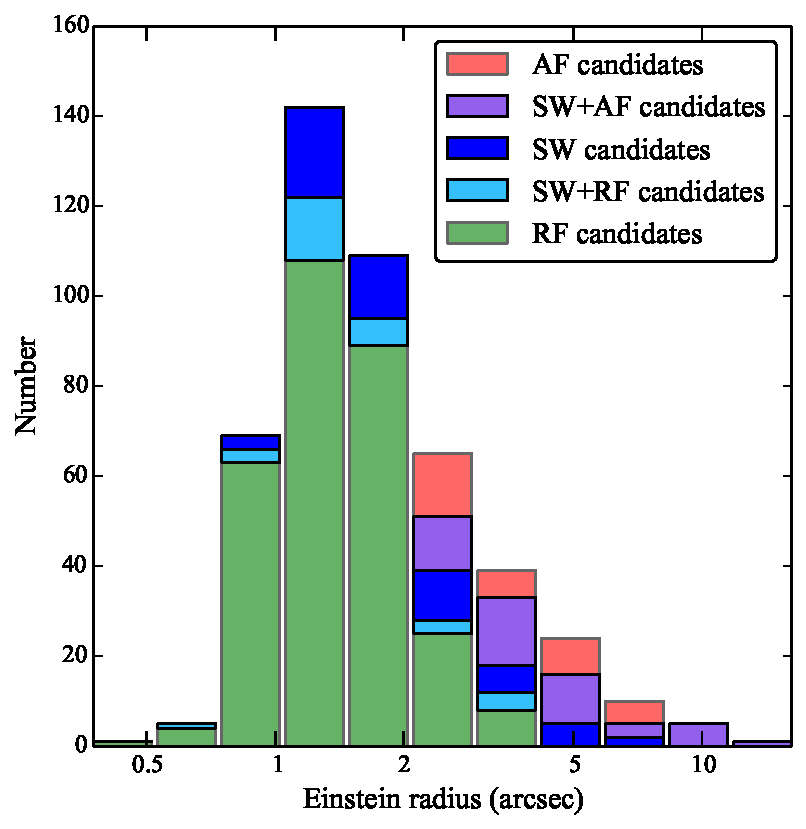
\includegraphics[scale=0.5]{sw-cfhtls-figs/stacked_lenscand_rein.pdf}
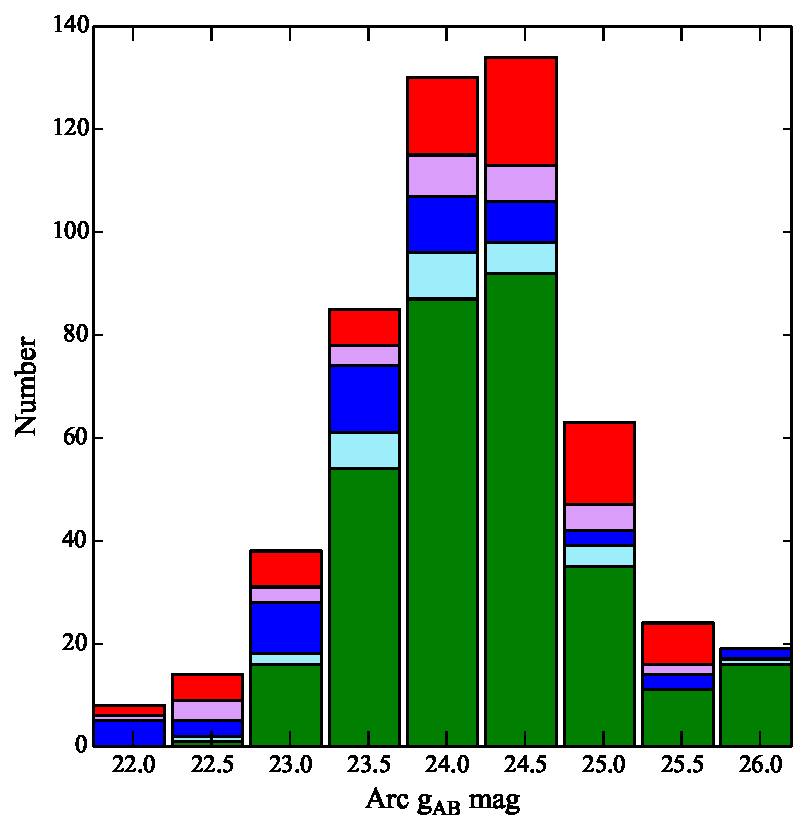
\includegraphics[scale=0.5]{sw-cfhtls-figs/stacked_lenscand_mag.pdf}
\caption{ \label{fig:stackremg}
Candidate detections by the \rf, \sw and the \af as a
function of the Einstein radius and $g$ band magnitude of the lensed
images.
%(XXXX check how different are the estimates from the different measurement techniques for a given lens candidates.)
}
\end{center}
\end{figure*}

In the following steps, the flux from the galaxy is subtracted from the
scaled difference image to enhance the visibility of the faint blue
lensed features. An object finder is run on this image to quantify the
lensed image properties. About 50\% of the \sw candidates could not be
detected by the object finder because properties such as the image area,
axis ratio, magnitude/color and alignment with respect to the lensing
galaxy are not satisfied. Some of the candidates missed at this stage
are, for example, SW4, SW5, SW6, SW25, SW35, SW38 and SW45.

%% 23/61 miss first step, 30/61 miss auto, 5 pass auto but have poor
%grade from visual classf.

Next, we rerun the \af on the same \sw sample of new candidates. The \af
is directly run on images to look for elongated arc like objects and does
not require a list of targets to begin with. Objects are identified by
placing thresholds on the noise level in the images. Thus, \af
detections are sensitive to changes in the noise levels.

Originally, the \af was run on a large image with an area of $\sim 19350
\times 19350$ pixels$^2$. For the rerun, we work with much smaller
images because this is faster but this alters the measured
noise and hence, affects the number and type of arc detections. We find
that about 30\% of the new candidates are detected without changing any
of the thresholds in the code because of the change in the noise level.
%{\bf does this make sense?}

The \af code calculates second order brightness moments around every
pixel to decide if the distribution of flux is elongated in some
direction in order to detect elongated arc-like objects. An elongation
estimator is assigned to every pixel. All pixels with a value of the
elongation stimator above a certain threshold are connected to form the arc
feature. This is building of the arc candidate. Subsequently, arc
properties such as the area, mean flux, length and curvature are
determined. We relax the threshold at the building stage and also relax
thresholds mainly on the area of the arc which leads to detection of
about 75\% of the new \sw candidates. We find that relaxing thresholds
on other arc properties do not improve the detection rate significantly
and thus are left unchanged.

Typically, the candidates are missed from the \af sample if a) they are
brighter in the redder band rather than the bluer $g$ band used for arc
detection because then the arc feature will be at the noise level and
will fail detection b) the flux of the arc and the galaxy are
blended in the $g$ band such that the \af mistakenly connects part of the
galaxy to the pixels belonging to the arc candidate which then results in a
candidate with no morphological characteristics of an arc or c) if the
candidate is not elongated which means most of the lensed quasars with
circular looking lensed images will be missed.

Relaxing the thresholds obviously increases the total number of
candidate detections which includes a large sample of false positives.
For example, the number of arc candidate detections increase by a factor
of $\sim$2 when we relaxed the thresholds in the reruns described above
whereas the number of false positives increase by a factor of $\sim$5.
Thus, it is not recommended to relax these thresholds alone. A better
alternative is to relax the thresholds to increase the completeness and
cross-correlate the arc candidate positions with a galaxy catalog to
discard those candidates which are not close to a putative lensing
galaxy within typical radius in order to reduce the false positives.

%% 19,46 (original and relaxed criteria); 72,338 (smaller image); 1548,7845 (larger image)


% % % % % % % % % % % % % % % % % % % % % % % % % % % % % % % % % % % % % % %

\subsection{False negatives: known lenses missed by \sw}
\label{sec:fn}
Like any lens finding method, the \sw system can fail to detect certain
kinds of lenses.  We find that about 40\% of the known sample of lenses
are missed both at \StageOne and II (see \Tref{tab:stats}). In fact, most
of the known lenses from \StageOne are discovered at \StageTwo suggesting
that most lenses are lost right at \StageOne. Below, we focus on the known
lens sample at \StageOne to understand why some of them are being missed
and possibly find a way to improve the detection rate which can be
adopted in the future \sw lens searches.

Many of the missed lenses are from the \rf sample with small
Einstein radii and faint lensed images (see \Fref{fig:compre}). Among
the confirmed lenses from the \rf, about 50\% are missed. Out of the
missed sample of 18 lenses, about half of them are visually difficult to
detect and the other half appear to have faint blue smudges around
galaxies which should have been easier to identify. Similarly,
if we consider the \af lens sample, $\sim$23\% are missed by \sw. This
is a relatively small sample of $\sim 5$ systems and visual inspection
suggests that, by and large, either the lensed features are faint
or they have odd properties which makes them difficult to identify
correctly. For further tests, we combine the \rf and \af sample.

For a lens finding method which uses collective skill, experience and
knowledge of a group of volunteers, it may be difficult to find a single
factor with certainty which causes a lens candidate to be missed. We
attempt to understand whether there is indeed a single dominant factor
that is resulting in the loss of these lenses or the lenses are being
missed due to a combination of multiple reasons. Below, we consider some
of the factors that could affect the efficiency of finding lenses.

\subsubsection{Number of classifications}
First, we check if the number of classifications (Nclass) is
significantly lower for the missed sample compared to the detected one.
Surprisingly, most of the lenses in the known sample have few
classifications (Nclass$<$10) which includes both the detected and
missed lenses. Many of the remaining lenses have between 10 to 20
classifications. And, only a few subjects have Nclass$>$20. They
continue to remain for long in the database because these candidates are
possibly difficult to identify. Therefore, the distribution of Nclass
can not be the reason for losing the lenses from the missed sample.

%{ Let us compare the two samples to see if there are any obvious differences. only 2 out of this sample of 18 were detected at \StageOne (reached high P even with fewer classifications) and missed at \StageTwo (P value was low even after recieving very many classifications). The rest of the 16 lenses were rejected right at \StageOne XXX}
%One of those 6 lenses was detected at \StageOne but failed to get high enough P value at \StageTwo even after receiving a total of 50 classifications (set as the upper limit). The rest of the 5 lenses are already rejected at \StageOne. Upon visual inspection of these 5 systems, they appear to be difficult to identify as lenses because either the lensed images are faint, have low curvature, are close to the edge and/or are not visible due to proximity to an extremely bright galaxy

\subsubsection{Blind lens search}
Efficiency of a visual search can vary in different sections of an
image. Our eyes tend to focus usually at the center of an image and lens
candidates close to the borders could go undetected. Therefore, it is
essential to test and understand if \sw is missing some of the known lenses
because they happen to be close to the borders of the image cutouts.

From the SWAP, the image cutouts inspected by the \sw volunteers receive
a status of detected (if P$>$P$_{\rm acc thresh}$), rejected (if
P$<$P$_{\rm rej thresh}$) and undecided (if P$_{\rm rej thresh}<$ P $<$
P$_{\rm acc thresh}$). In \Fref{fig:comppos}, we compare the positions
of lenses which are detected (red), undecided (green) and rejected
(blue). The left and the right panels have the simulated lens sample and
the known lens candidates sample, respectively. We note that the density
of points do not represent the actual number of detections because, for some
cases, randomly selected subsamples are shown for the ease of visual
comparison.

We do not find any strong visual correlation in the detection rate of
lenses as a function of their positions in the image for both the
simulated and the known lens sample. Thus, the completeness of the lens
sample is most likely not significantly affected by whether a lens is
located close to the border or well within the center.

\subsubsection{Volunteer profile}

Here, we investigate if the power\footnote{see the
\Aref{appendix:power} for the meaning of this term and how it is
different from the ``Skill'' defined in paper I} of volunteers is systematically
different between the sample of detected and missed lenses.

We check how the posterior probability P (see Paper I for the
mathematical definition) of an image or a subject to contain a lens
changes as the image receives more classifications from multiple
volunteers.  In \Fref{fig:detmis}, we show the trajectory plots of a few
examples of detected lenses (top left panels) and missed lenses (bottom
left panels) by \sw at \StageOne. The number of classifications (Nclass)
for a subject increase from top to bottom.  Also, every subject is
assigned a prior probability P0$=2\times10^{-4}$ (grey dashed line) and
starts at the middle of the trajectory plot. The P value of a subject is
updated with every classification from the volunteer.  If a volunteer
identifies a lens candidate, the trajectory moves to the right otherwise
moves to the left. A subject is accepted if it crosses the blue-dashed
line marking the (P$_{\rm acc thresh}=0.95$) on the right and is
rejected, if it crosses the red-dashed line marking the P$_{\rm rej
thresh}=10^{-7}$ on the left.

By how much the P value will change depends on how well the
volunteers are performing on the training sample. Thus, high power
volunteers will change the P by a large factor compared to the low
power volunteers. This is evident in the trajectory plots as large and
small distances in between the consequent points which we refer to as
kicks. Comparison of the kick sizes between the detected
and the missed lenses suggests that the missed lenses do not have as
many volunteers giving large kicks. We also note that most of the large
kicks seen in the trajectories of the missed lenses seem to be moving
the subjects to the right. In other words, the high power volunteers
are mostly classifying them as subjects with lens candidates. Further
qualitative comparison and discussion of the trajectory plots is given
in \Aref{appendix:traj}.

For a quantitative comparison of the large and small kicks for the
entire samples of detected and missed known lenses, we show a plot of
histogram on the right of \Fref{fig:detmis}. Qualitatively, there are
four types of volunteers making classifications - those causing positive
large kicks (correct classifications by high power volunteers, those
causing positive small kicks (correct classifications by low power
volunteers), those causing negative small kicks (incorrect
classifications by low power volunteers) and those causing negative
large kicks (incorrect classifications by high power volunteers). The
four histograms in the figure correspond to these four types of
volunteers for each sample (that is, detected or missed). The kick size
is small if $\Delta$ log(P)$=$log (P$_{\rm current}) - $log(P$_{\rm
previous}) < \Delta$log(P)$_{\rm cut}$ (chosen to be 1.2) and is large
if greather than $\Delta$log(P)$_{\rm cut}$.

Some of the key differences are i) the ratio of positive large kicks to
positive small kicks for the detected sample is higher than the missed
sample suggesting that the fraction of high power volunteers is large
for the detected sample ii) in terms of Nclass, the missed sample is
dominated by volunteers causing negative small kicks whereas for the
detected sample there is a comparable contribution from three types of
volunteers - positive small and large kicks and negative small kicks.
iii) the Nclass from volunteers with negative large kicks are lower both
for the detected and the missed samples. this is consistent with our
expectation that high power volunteers should not be making incorrect
classifications.Therefore, lack of high power volunteers classifying
the missed lenses seems to be one of the major factors.

We rerun SWAP for \StageOne where we use classifications from volunteers
who produce $\Delta$ log(P)$>1.2$ only. This obviously means reducing
the total Nclass per subject by a large fraction. As a result, we also
need to change the P$_{\rm acc thresh}$ which is chosen to be 0.1 and we
find that about a third of the missed lenses are detected while all the
previously detected lenses remain detected too. The others simply do not
have enough classifications from volunteers producing large positive
kicks. Thus, it may be possible to detect more promising candidates if
we preferentially show the rejected systems to a few high power
volunteers. We understand that changing the rejection and acceptance
thresholds will likely increase the rate of FPs along with
improved completeness but most probably the increase in FPs will not be
too significant and that it will still be worth using the new strategy.


\begin{figure*}
\begin{center}
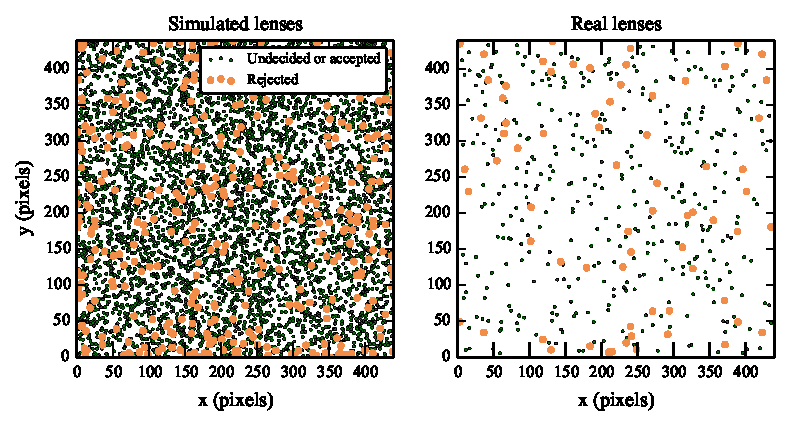
\includegraphics[scale=0.95]{sw-cfhtls-figs/completeness_pos.pdf}
\caption{ \label{fig:comppos}
Completeness as a function of the positions of the lens systems. Simulated lenses
(left) and real lens candidates (right) are shown. Irrespective of the
status of the lenses, that is, detected, undecided or rejected, there is
no strong dependency on the location of the lenses, both for the
simulated and the real sample of candidates. }
\end{center}
\end{figure*}


\begin{figure*}
\begin{center}
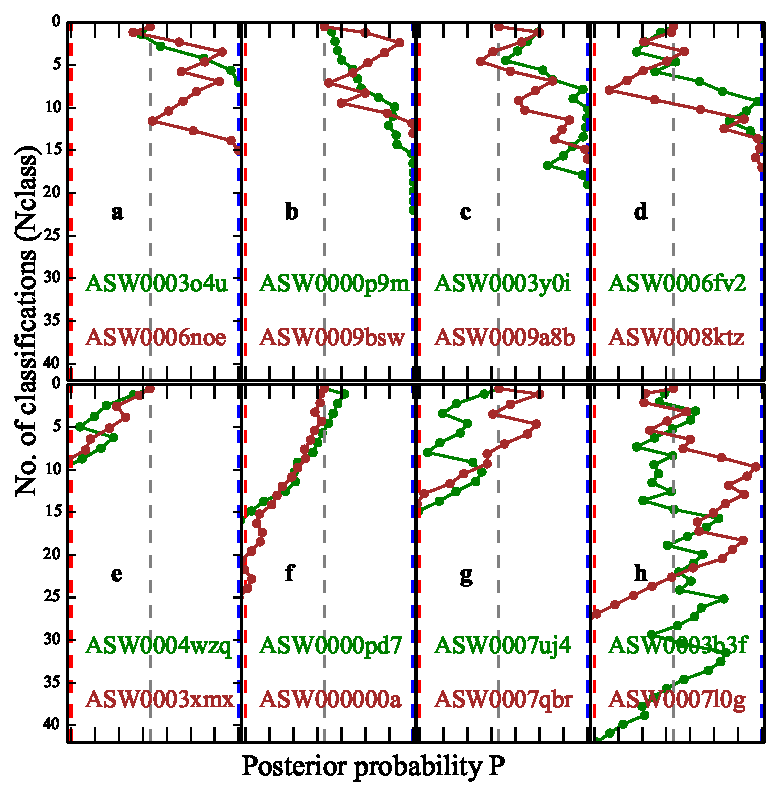
\includegraphics[scale=0.6]{sw-cfhtls-figs/det_mis_traj.pdf}
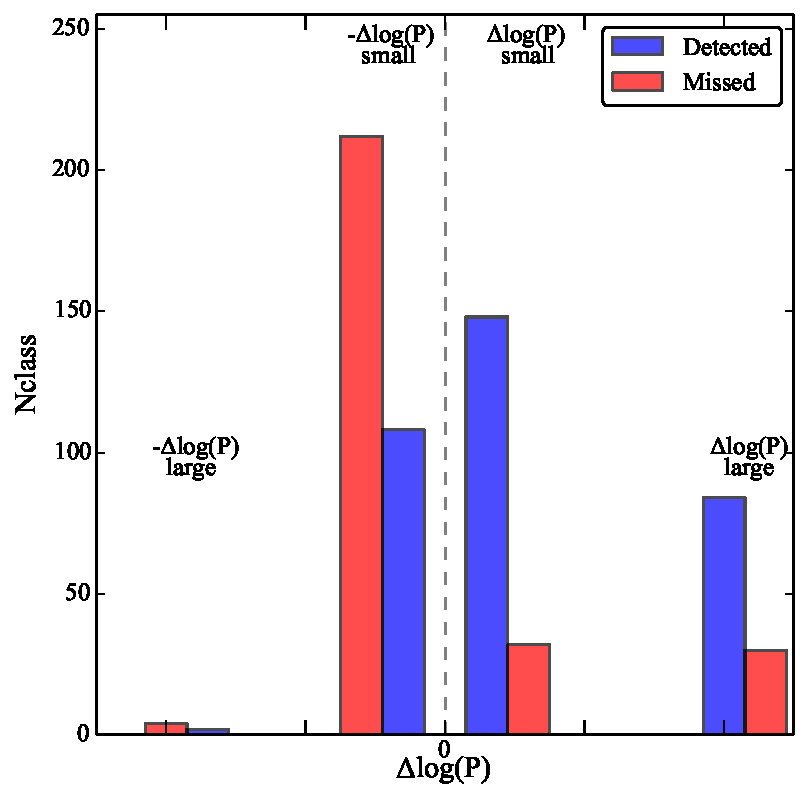
\includegraphics[scale=0.6]{sw-cfhtls-figs/det_mis_hist.pdf}
\caption{ \label{fig:detmis}
Examples of trajectories of some known lenses (top-left: detected and
bottom-left: missed) at \StageOne and histogram of the known lenses for
different types of volunteers (right). Among the sample of missed
lenses, most classifications are from the low power volunteers
identifying these images incorrectly (i.e. $-\Delta$~logP) which
overshadows the small number of correct identifications (i.e.
$\Delta$~logP) coming from both the less and the high power volunteers
combined. For the detected lens sample, most classifications are correct
identifications coming from both low and high power volunteers.
}
\end{center}
\end{figure*}


%%%%%%%%%%%%%%%%%%%%%%%%%%%%%%%%%%%%%%%%%%%%%%%%%%%%%%%%%%%%%%%%%%%%%%%%%%%%%%

\section{Summary and Conclusions}
\label{sec:conclude}

We report the discovery of new gravitational lens candidates from the
the first lens search through \sw. In this search, volunteers are shown
$g-r-i$ color images of random regions of the sky taken by the CFHT Legacy
Survey. The aim of this blind lens search is to find lenses that have been
missed by previous searches done on the \cfhtls with lens finding
algorithms. In this search, we use a training sample to train the
volunteers and calibrate their performance which helps us in more
efficient pruning of the lens candidates. The training sample has
simulated lenses, duds and FPs. In this paper, we describe the details
of the training sample generated and tuned for the \cfhtls data.
Volunteers receive feedback messages when they click or fail to click on
the training images during live classification of real images which
helps them remain focused and improve their performance over time. More
details about the design of \sw system and how it works are given in the
companion paper, Paper I.

The blind lens search in the \cfhtls is done in two stages: \StageOne and
\StageTwo. In \StageOne, volunteers inspected $\sim$ 430 000 subjects and
selected a smaller sample of $\sim$ 3000 subjects with interesting lens
candidates. In \StageTwo, after a careful reinspection of the candidates
from \StageOne, a smaller pool of more pure sample of $\sim$~500
candidates is obtained. In the next step, the images are graded by three
lens experts (AM, AV and PJM) producing candidates that range from
mildly interesting to certainly a lens system.

In this paper (Paper II), we present the new \sw sample and compare this
with the previously known samples from two robotic searches from the
\cfhtls namely, the \rf and \af. And, further details about the new
sample such as any follow up confirmation and investigations including
mass modelling analysis will be presented in a subsequent \sw paper
(Paper III). 

Below, we give some of our conclusions from the first \sw lens search
and the comparison with robotic searches:
\begin{itemize}

\item \sw works well as a discovery engine for gravitational lenses
through citizen science. While a targeted visual search may be more
efficient, we show that the blind search works reasonably well too.

\item We present a sample of 58 {\bf new} gravitational lens candidates
out of which 28 are more promising systems. These candidates received
averaged grades, G$\ge$1.3 from three experts where 1-mildly interesting,
2-probably, a lens and 3-certainly, a lens. Another sample of over 100
lens candidates is recovered from previously known samples of lens
candidates.

\item Compared to the sample of robotically (the \rf and \af) detected
lens candidates, the \sw sample finds lens systems with similar range in
the lens redshift and properties of the lensed images such as the total
magnitude and the Einstein radii. However, the \sw search being a purely
visual one cannot find some of the \rf-identified-lensed images with
sub-arcsecond Einstein radii because the flux of the typically faint
lensed images is obscured by the flux from bright lensing galaxies. The
\rf finds these candidates because it works with lensing
galaxy-subtracted images.

\item Qualitatively, the \sw sample finds lens systems with different
types of lensing galaxies, for example, elliptical, spiral (face on and
edge on) and small red galaxies unlike those found from robotic
searches. Similarly, the lensed images too have different colors,
morphologies and sizes which are again typically missed by any given
algorithm.

\item Based on the known sample of lenses and lens candidates, we find
that we lose a very small fraction of them as we go from \StageOne to
\StageTwo. In other words, it is more important to improve the lens
detection efficiency right at \StageOne to increase the overall
completeness of the final lens sample

\item From the sample of known lenses, \sw missed about 40\% at \StageOne.
Among the missed sample of about 20 lenses, roughly half of them are
visually difficult to identify because most of them are faint with small
image separations which are identified through the \rf

\item If we use the classifications from more skilled volunteers alone
at \StageOne, then we recover over 30\% of the lenses from the missed
sample. Thus, it is possible to improve the completeness of lenses by
changing the strategy of when and who is shown an image.

\end{itemize}


\onecolumn
\begin{center}
\begin{longtable}{llrrrrrrlrr}
\caption{ \label{tab:swcands}
Sample of the \sw new lens candidates. }\\
\hline
SW ID & Name & RA & Dec &  $z_{\rm phot}$ & $m_i$ & $R_{\rm A}$ & G & ZooID & P & Comments  \\
  &  & (deg) & (deg) &  & (mag) &  (") &  &  & & \\
\hline
\endfirsthead
\hline
SW ID & Name & RA & Dec &  $z_{\rm phot}$ & $m_i$ & $R_{\rm A}$ & G & ZooID & P & Comments  \\
  &  & (deg) & (deg) &  & (mag) &  (") &  &  & & \\
\hline
\endhead
\hline
\multicolumn{11}{p{18cm}}{
The column Comments has two type of notes. The first is about the lens
image configuration where the symbols mean the following A: Arc, D: Double, Q:
Quad, R: Ring. The second is a comment on the type of lens assessed
visually. Note that this classification is not based on colors or spectral
analysis. The symbols are E: Elliptical, S: (face on) Spiral, G: Group-scale, D:
Edge on disk, R: Red starforming galaxy.  This galaxy falls within the masked region as per the catalog from
which the magnitudes and the redshift are extracted.
%{\bf Note:} $\dagger$ are systems found in \citet{Gavazzi2014} as part of the additional
%sample and $\ast$ is found in \citet{Maturi2014} sample.
}\\
\endlastfoot
 SW1 & CFHTLS J022409-105807 &   36.0398 &  -10.9688 &  0.0 &  0.0 &  4.8 &  3.0 & ASW0004dv8 &  1.0  &  A,G   \\
 SW2 & CFHTLS J140522+574333 &  211.3426 &   57.7259 &  0.7 & 19.7 &  1.0 &  2.7 & ASW000619d &  0.7  &  A,R   \\
 SW3 & CFHTLS J142603+511420 &  216.5149 &   51.2390 &  0.0 &  0.0 &  4.4 &  2.7 & ASW0006mea &  0.7  &  A,G   \\
 SW4 & CFHTLS J142934+562541 &  217.3926 &   56.4281 &  0.5 & 19.0 &  5.9 &  2.7 & ASW0009cjs &  0.8  &  A,G   \\
 SW5 & CFHTLS J143454+522850 &  218.7270 &   52.4808 &  0.6 & 19.4 &  4.4 &  2.7 & ASW0007k4r &  0.4  &  Q,G/R   \\
 SW6 & CFHTLS J143627+563832 &  219.1164 &   56.6425 &  0.5 & 19.4 &  1.5 &  2.7 & ASW0008swn &  0.9  &  A,D   \\
 SW7 & CFHTLS J220256+023432 &  330.7369 &    2.5758 &  0.0 &  0.0 &  6.8 &  2.7 & ASW0007e08 &  0.8  &  A,G/C   \\
 SW8 & CFHTLS J020832-043315 &   32.1340 &   -4.5543 &  1.0 & 21.0 &  1.6 &  2.3 & ASW0002asp &  1.0  &  A,R   \\
 SW9 & CFHTLS J020848-042427 &   32.2011 &   -4.4075 &  0.8 & 20.5 &  1.1 &  2.3 & ASW0002bmc &  0.9  &  D,D   \\
SW10 & CFHTLS J020849-050429 &   32.2078 &   -5.0749 &  0.8 & 20.6 &  0.9 &  2.3 & ASW0002qtn &  1.0  &  A,R   \\
SW11 & CFHTLS J022406-062846 &   36.0256 &   -6.4796 &  0.4 & 19.6 &  0.9 &  2.3 & ASW0003wsu &  0.7  &  A,E   \\
SW12 & CFHTLS J022805-051733 &   37.0236 &   -5.2927 &  0.4 & 18.8 &  1.4 &  2.3 & ASW0009ans &  1.0  &  Q,E   \\
SW13 & CFHTLS J023123-082535 &   37.8468 &   -8.4266 &  0.0 &  0.0 &  1.2 &  2.3 & ASW0004xjk &  0.3  &  A,R   \\
SW14 & CFHTLS J084841-045237 &  132.1708 &   -4.8772 &  0.3 & 19.0 &  1.0 &  2.3 & ASW0004nan &  1.0  &  A,E   \\
SW15 & CFHTLS J140030+574437 &  210.1260 &   57.7437 &  0.4 & 18.2 &  2.0 &  2.3 & ASW0009bp2 &  0.6  &  A,E   \\
SW16 & CFHTLS J140622+520942 &  211.5958 &   52.1617 &  0.7 & 20.3 &  1.2 &  2.3 & ASW0005rnb &  0.7  &  A,R   \\
SW17 & CFHTLS J143658+533807 &  219.2425 &   53.6355 &  0.7 & 19.6 &  0.9 &  2.3 & ASW0007hu2 &  0.6  &  D,D   \\
SW18 & CFHTLS J020642-095157 &   31.6750 &   -9.8658 &  0.2 & 20.8 &  0.9 &  2.0 & ASW0001ld7 &  0.8  &  A,R   \\
SW19 & CFHTLS J021221-105251 &   33.0881 &  -10.8811 &  0.3 & 17.9 &  1.8 &  2.0 & ASW0002dx7 &  0.8  &  D,E/S   \\
SW20 & CFHTLS J022533-053204 &   36.3888 &   -5.5346 &  0.5 & 19.4 &  3.6 &  2.0 & ASW0004m3x &  0.4  &  A,R/G   \\
SW21 & CFHTLS J022716-105602 &   36.8186 &  -10.9341 &  0.4 & 17.2 &  1.8 &  2.0 & ASW0009ab8 &  0.7  &  A,E/G   \\
SW22 & CFHTLS J023008-054038 &   37.5359 &   -5.6774 &  0.6 & 19.7 &  1.9 &  2.0 & ASW0003r61 &  0.5  &  A,E   \\
SW23 & CFHTLS J023315-042243 &   38.3133 &   -4.3789 &  0.7 & 19.7 &  1.0 &  2.0 & ASW00050sk &  0.8  &  A,R   \\
SW24 & CFHTLS J090308-043252 &  135.7844 &   -4.5479 &  0.0 &  0.0 &  1.2 &  2.0 & ASW00007mq &  0.6  &  A,E   \\
SW25 & CFHTLS J135755+571722 &  209.4827 &   57.2897 &  0.8 & 20.2 &  1.3 &  2.0 & ASW0005ma2 &  0.8  &  D,D   \\
SW26 & CFHTLS J141432+534004 &  213.6372 &   53.6679 &  0.7 & 21.4 &  0.9 &  2.0 & ASW0006jh5 &  0.8  &  A,R   \\
SW27 & CFHTLS J143055+572431 &  217.7333 &   57.4088 &  0.7 & 19.3 &  1.0 &  2.0 & ASW0007wfj &  0.9  &  A,R   \\
SW28 & CFHTLS J143838+572647 &  219.6589 &   57.4464 &  0.8 & 20.2 &  1.1 &  2.0 & ASW0008qsm &  0.9  &  A,R   \\
SW29 & CFHTLS J021057-084450 &   32.7414 &   -8.7474 &  0.0 &  0.0 &  2.5 &  1.7 & ASW0002p8y &  0.4  &  A,G   \\
SW30 & CFHTLS J021514-092440 &   33.8109 &   -9.4111 &  0.7 & 19.9 &  2.6 &  1.7 & ASW00021r0 &  0.4  &  A,R/G   \\
SW31 & CFHTLS J022359-083651 &   35.9995 &   -8.6143 &  0.0 &  0.0 &  3.1 &  1.7 & ASW0004iye &  0.4  &  A,E   \\
SW32 & CFHTLS J022745-062518 &   36.9387 &   -6.4218 &  0.6 & 20.5 &  1.2 &  1.7 & ASW0003s0m &  0.5  &  A,R   \\
SW33 & CFHTLS J023453-093032 &   38.7232 &   -9.5089 &  0.5 & 19.8 &  0.7 &  1.7 & ASW00051ld &  0.3  &  A,D   \\
SW34 & CFHTLS J084833-044051 &  132.1385 &   -4.6809 &  0.8 & 20.2 &  0.9 &  1.7 & ASW0004wgd &  0.7  &  A,R   \\
SW35 & CFHTLS J090248-010232 &  135.7020 &   -1.0424 &  0.4 & 19.1 &  1.4 &  1.7 & ASW000096t &  0.6  &  D,E   \\
SW36 & CFHTLS J143100+564603 &  217.7511 &   56.7675 &  0.0 &  0.0 &  1.8 &  1.7 & ASW00086xq &  0.8  &  A,E   \\
SW37 & CFHTLS J143353+542310 &  218.4736 &   54.3862 &  0.8 & 19.8 &  1.6 &  1.7 & ASW0009cox &  0.6  &  A,R/G   \\
SW38 & CFHTLS J220215+012124 &  330.5635 &    1.3567 &  0.3 & 17.4 &  4.6 &  1.7 & ASW0005qiz &  0.5  &  rA,G   \\
SW39 & CFHTLS J221306+014708 &  333.2758 &    1.7856 &  0.0 & 17.1 &  1.4 &  1.7 & ASW0008wmr &  0.9  &  A,S   \\
SW40 & CFHTLS J221519+005758 &  333.8321 &    0.9661 &  0.4 & 20.2 &  1.0 &  1.7 & ASW0008xbu &  0.8  &  A,D   \\
SW41 & CFHTLS J221716+015826 &  334.3189 &    1.9739 &  0.1 & 21.6 &  1.0 &  1.7 & ASW00096rm &  1.0  &  A/R,R   \\
SW42 & CFHTLS J020810-040220 &   32.0450 &   -4.0389 &  1.0 & 20.8 &  1.8 &  1.3 & ASW0001c3j &  0.7  &  A,R   \\
SW43 & CFHTLS J021021-093415 &   32.5898 &   -9.5711 &  0.4 & 18.4 &  2.7 &  1.3 & ASW0002k40 &  0.4  &  D,S   \\
SW44 & CFHTLS J021225-085211 &   33.1051 &   -8.8697 &  0.8 & 19.5 &  2.1 &  1.3 & ASW00024id &  1.0  &  R,R   \\
SW45 & CFHTLS J021317-084819 &   33.3234 &   -8.8055 &  0.5 & 19.8 &  1.3 &  1.3 & ASW00024q6 &  0.4  &  A,R/E   \\
SW46 & CFHTLS J022843-063316 &   37.1794 &   -6.5547 &  0.5 & 19.1 &  1.8 &  1.3 & ASW0003r6c &  0.3  &  D/A,E   \\
SW47 & CFHTLS J090219-053923 &  135.5794 &   -5.6566 &  0.0 &  0.0 &  2.0 &  1.3 & ASW0000g95 &  1.0  &  A,R/E   \\
SW48 & CFHTLS J090319-040146 &  135.8311 &   -4.0297 &  0.0 & 19.8 &  1.2 &  1.3 & ASW00007ls &  0.5  &  A,R/E   \\
SW49 & CFHTLS J090333-005829 &  135.8886 &   -0.9749 &  0.0 &  0.0 &  2.1 &  1.3 & ASW00008a0 &  1.0  &  A/D,E/G   \\
SW50 & CFHTLS J135724+561614 &  209.3536 &   56.2707 &  0.0 &  0.0 &  2.6 &  1.3 & ASW0006e0o &  0.9  &  D,E   \\
SW51 & CFHTLS J140027+541028 &  210.1164 &   54.1746 &  0.0 &  0.0 &  1.2 &  1.3 & ASW0006a07 &  0.6  &  Q,R/E   \\
SW52 & CFHTLS J141518+513915 &  213.8290 &   51.6542 &  0.4 & 18.3 &  3.0 &  1.3 & ASW00070vl &  0.8  &  D,E   \\
SW53 & CFHTLS J142620+561356 &  216.5870 &   56.2323 &  0.5 & 19.5 &  1.3 &  1.3 & ASW0007sez &  0.8  &  A/R,S   \\
SW54 & CFHTLS J142652+560002 &  216.7201 &   56.0006 &  0.0 &  0.0 &  1.5 &  1.3 & ASW0007t5y &  1.0  &  R,R   \\
SW55 & CFHTLS J142843+543713 &  217.1815 &   54.6204 &  0.4 & 19.7 &  1.3 &  1.3 & ASW0007pga &  0.6  &  D,D   \\
SW56 & CFHTLS J143631+571131 &  219.1315 &   57.1922 &  0.7 & 20.9 &  1.3 &  1.3 & ASW0008pag &  0.6  &  D/A,R   \\
SW57 & CFHTLS J143651+530705 &  219.2150 &   53.1183 &  0.6 & 19.2 &  3.1 &  1.3 & ASW0007h27 &  1.0  &  A,E/G   \\
SW58 & CFHTLS J143950+544606 &  219.9609 &   54.7686 &  0.0 &  0.0 &  1.7 &  1.3 & ASW00085cp &  0.4  &  A,G/R   \\

\end{longtable}
\end{center}

%%SW23$^{\dagger}$ & CFHTLS J023051-082423 &   37.7141 &   -8.4064 &  0.0 &  0.0 &  0.8 &  2.0 & ASW000412m &  0.4  &  A,E   \\
%%SW41$^{\ast}$ & CFHTLS J221513+010240 &  333.8056 &    1.0446 &  0.0 &  0.0 &  0.8 &  1.7 & ASW0008dxh &  0.3  &  A,R/G   \\
%%SW54$^{\dagger}$ & CFHTLS J140425+520506 &  211.1062 &   52.0850 &  0.4 & 18.9 &  1.4 &  1.3 & ASW0005o0w &  0.6  &  D,E   \\
\twocolumn
%%%%%%%%%%%%%%%%%%%%%%%%%%%%%%%%%%%%%%%%%%%%%%%%%%%%%%%%%%%%%%%%%%%%%%%%
%%  ACKNOWLEDGMENTS
%%%%%%%%%%%%%%%%%%%%%%%%%%%%%%%%%%%%%%%%%%%%%%%%%%%%%%%%%%%%%%%%%%%%%%%%
\section*{Acknowledgements}

We thank all \Ncollaboration members of the \sw community for their
contributions to the project so far. A complete list of collaborators is
provided at \texttt{http://spacewarps.org/\#/results/CFHTLS}.

We are also grateful to Stuart Lynn, Kelly Borden, Laura Whyte, Brooke Simmons,
David Hogg, Thomas Jennings, Layne  Wright, Cecile Faure, Jonathan Coles, Stuart
Lowe and Jean-Paul Kneib for many useful conversations about citizen science and
gravitational lens detection, and to the Dark Energy Survey and Pan-STARRS strong
lensing science teams for their suggestions and encouragement.

PJM was given support by the Royal Society, in the form of a research
fellowship, and by the U.S. Department of Energy under contract number DE-AC02-76SF00515.
%
AV acknowledges support from the Leverhulme Trust in the form of a research
fellowship.
%
The work of AM and SM was supported by World Premier International Research
Center Initiative (WPI Initiative), MEXT, Japan. The work of AM was also supported in
part by National Science Foundation Grant No. PHYS-1066293 and the hospitality
of the Aspen Center for Physics.
%
% Zooniverse / Sloan Foundation.
%
% Other authors.
PJM and ES thank the Institute of Astronomy and Astrophysics, Academia Sinica
(ASIAA) and Taiwan's Ministry of Science and Technology (MOST) for their
financial support of the workshop ``Citizen Science in Astronomy'' in March
2014, at which some parts of the SWAP analysis was developed.

The \sw project is open source.
The web app was developed at \texttt{https://github.com/Zooniverse/Lens-Zoo}, and was supported by a grant from the Alfred P. Sloan Foundation, 
while the SWAP analysis software was developed at
\texttt{https://github.com/drphilmarshall/SpaceWarps}.

The CFHTLS data used in this work are based on observations obtained with
MegaPrime/MegaCam, a joint project of CFHT and CEA/IRFU, at the
Canada-France-Hawaii Telescope (CFHT) which is operated by the National Research
Council (NRC) of Canada, the Institut National des Science de l'Univers of the
Centre National de la Recherche Scientifique (CNRS) of France, and the
University of Hawaii. This work is based in part on data products produced at
Terapix available at the Canadian Astronomy Data Centre as part of the
Canada-France-Hawaii Telescope Legacy Survey, a collaborative project of NRC and
CNRS.

This work is based on observations obtained with MegaPrime/MegaCam, a joint
project of CFHT and CEA/IRFU, at the Canada-France-Hawaii Telescope (CFHT) which
is operated by the National Research Council (NRC) of Canada, the Institut
National des Sciences de l'Univers of the Centre National de la Recherche
Scientifique (CNRS) of France, and the University of Hawaii. This research used
the facilities of the Canadian Astronomy Data Centre operated by the National
Research Council of Canada with the support of the Canadian Space Agency.
CFHTLenS data processing was made possible thanks to significant computing
support from the NSERC Research Tools and Instruments grant program.

%%%%%%%%%%%%%%%%%%%%%%%%%%%%%%%%%%%%%%%%%%%%%%%%%%%%%%%%%%%%%%%%%%%%%%%%%%%%%%
%  APPENDICES
%%%%%%%%%%%%%%%%%%%%%%%%%%%%%%%%%%%%%%%%%%%%%%%%%%%%%%%%%%%%%%%%%%%%%%%%%%%%%%

\appendix

\section{Qualitative comparison of detected and missed known lenses}
\label{appendix:traj}

The bottom panels show the missed or rejected lenses. The green (and red)
trajectories show visually easier (and more difficult) to identify
lenses. In spite of some mild qualitative differences, both set of
trajectories have very similar behaviour. The trajectories in panel e
are typical of this sample in terms of Nclass and the dominance of short
negative kicks. The panel f represents a small fraction of this sample
where the kics are only short and negative. The panel g shows how some
lenses receive a bunch of large positive kicks which are led to
rejection by still mostly negative short kicks. Finally, panel h shows
those cases of lenses which received almost sufficient number of large
positive kicks to be detected but ended up being rejected.

The top panels show the detected lenses. The cases shown with green trajectories
in each panel can be thought of counterparts of the trajectories of the missed
lenses in the corresponding bottom panel except that the type of volunteers are
different. Most detected lenses are similar to the case in panel a which are
detected within a few classifications but coming from large positive kicks.
Panel b represents a few odd cases which are dominated mainly by short positive
kicks. Panel c shows a lens getting more classifications because of the tug
between positive and negative kicks whereas the panel d represents the extreme
cases when the subjects are on the verge of being rejected but are saved thanks
to a series of large positive kicks. The red trajectories are some more
examples of randomly selected cases which demonstrate how having sufficient
number of large positive kicks allows lenses to be detected in spite of several
short negative kicks.

\section{Lens Detection Power}
\label{appendix:power}

In \PaperOne, we defined the ``Skill'' of an agent as being given by the
expectation value of the information gain per classification. This
quantity is a non-linear function of both the $P_{\rm L}$, the
probability of correctly identifying a lens as a lens and $P_{\rm D}$,
the probability of correctly identifying a dud as a dud. This means that
one can get the same value of Skill for different combinations of
$P_{\rm L}$ and $P_{\rm D}$ (see the left panel of
\Fref{fig:skilldlnp}). The skill reflects the all-round ability of a
classifier to contribute information.

As described in the appendix of \PaperOne, the posterior probability $P$
of a subject is determined by the $P_{\rm L}$ and $P_{\rm D}$ of all the
volunteers who clicked on the subject, via Bayes' Theorem. Each agent
will apply a ``kick'' of a different size to the subject probability,
$\Delta\log(P)$, which can be either positive (if the classifier thinks
the subject contains a lens) or negative (if the classifier thinks the
subject does not contain a lens). For instance, given a subject
(not) containing a lens, a volunteer with high ($P_{\rm D}$) $P_{\rm L}$
implies a large (negative) positive kick irrespective the value of
($P_{\rm L}$) $P_{\rm D}$ as shown in the (right most) middle panel of
\Fref{fig:skilldlnp}. However, large (negative) positive kicks are
still possible for a volunteer located in the (lower) upper triangle
with different combinations of ($P_{\rm L}$,$P_{\rm D}$) suggesting that
the kick is not a simple function of ($P_{\rm L}$,$P_{\rm D}$).

The kicks appear as steps on the subject's trajectory plot. This kick
magnitude gives a useful measure of an agent's ``Power'' to move
subjects closer to detection.  Note that a volunteer who is very good at
rejecting duds, but not so good at identifying lenses, may have a high
Skill but a low Power (since they may fail to detect many of the
interesting lenses): Power provides a more precise quantification of a
classifier's ability to detect lenses (compared to rejecting non-lenses).


\begin{figure*}
\begin{center}
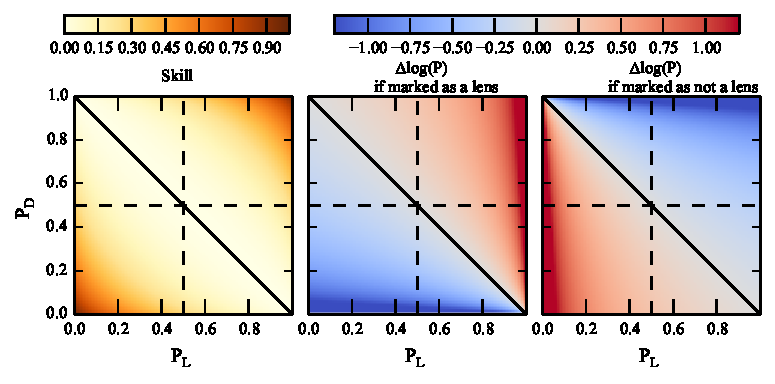
\includegraphics[scale=1.0]{sw-cfhtls-figs/dlnp_skill.pdf}
\caption{ \label{fig:skilldlnp}
Skill of the volunteers, $\Delta\log(P)$ given a lens or not a lens in
an image as a function of $P_{\rm L}$ and $P_{\rm D}$. Each of these
quantities represent ability of the Volunteers but do not have a simple
linear relation with $P_{\rm L}$ and $P_{\rm D}$.  
\question{AM}{PJM, should we just use power everywhere instead of the
$\Delta\log(P)$? This figure and this section still needs to be
polished.}
}
\end{center}
\end{figure*}


%{\bf todo: 
%check what happened to
%those AF lenses which were labelled sims - look at the D11 counterparts
%and their status in \StageOne swap}

%%{\bf there are 70 images which have both sims and known lenses. for
%the sims ID, 69 det and 1 rej (nearly 100% detected) whereas the
%corresponding test IDs 30det-30rej (nearly 50% detected and 50%lost) --
%what does this mean?}

%%%%%%%%%%%%%%

%%%%%%%%%%%%%%%%%%%%%%%%%%%%%%%%%%%%%%%%%%%%%%%%%%%%%%%%%%%%%%%%%%%%%%%%%%%%%%
%  REFERENCES
%%%%%%%%%%%%%%%%%%%%%%%%%%%%%%%%%%%%%%%%%%%%%%%%%%%%%%%%%%%%%%%%%%%%%%%%%%%%%%

% MNRAS does not use bibtex, input .bbl file instead.
% Generate this in the makefile using bubble script in scriptutils:

% bubble -f paper-lcr.tex references.bib
% \input{paper-lcr.bbl}

\bibliographystyle{apj}
%\bibliography{references}
\bibliography{references_cfhtls}


%%%%%%%%%%%%%%%%%%%%%%%%%%%%%%%%%%%%%%%%%%%%%%%%%%%%%%%%%%%%%%%%%%%%%%%%%%%%%%

\label{lastpage}
\bsp

\end{document}

%%%%%%%%%%%%%%%%%%%%%%%%%%%%%%%%%%%%%%%%%%%%%%%%%%%%%%%%%%%%%%%%%%%%%%%%%%%%%%
